\documentclass[a4paper, 12pt, twoside]{article}
\usepackage[english]{babel}
\usepackage[utf8]{inputenc}

%Margins
\usepackage[left=25.4mm, right = 25.4mm, top=25.4mm, bottom=25.4mm, includefoot]{geometry}

%For beautiful paragraph spacing
\usepackage{parskip}
\setlength{\parindent}{0in}
\usepackage{enumitem}
\usepackage{setspace}

%Adding Pictures
\usepackage{graphicx}
\usepackage{float}
\usepackage{pdflscape} %converts page from to portrait to landscape mode
\usepackage{wrapfig}


%Header and Footers
\usepackage{fancyhdr}
\pagestyle{fancy}
\fancyhead{}
\fancyfoot{}
\fancyfoot[RO]{Centre for Civil Society \hspace{1mm} \textbar \hspace{1mm} \thepage\ }
\fancyfoot[LE]{ \thepage \hspace{1mm} \textbar \hspace{1mm}SVAC Report 2018 }
\renewcommand{\headrulewidth}{0pt} %change the pt width to insert header line
\renewcommand{\footrulewidth}{0pt} %change the pt width to insert footer line

%Maths
\usepackage{amsmath}
\usepackage{mathtools}


%Tables
\usepackage{booktabs}
\usepackage{multicol}
\usepackage{subfig}
\captionsetup{aboveskip=14pt,}
\captionsetup[table]{singlelinecheck = false}
\usepackage{rotating}
\usepackage{longtable}
\usepackage[table]{xcolor}
\usepackage{makecell}
\renewcommand\theadfont{\scriptsize}
\usepackage{array}
\usepackage{cellspace}
\setlength\cellspacetoplimit{3pt}
\setlength\cellspacebottomlimit{3pt}

%Coloured Boxes
\usepackage{xcolor}
\usepackage{mdframed}


%Custom Spacing
\usepackage{setspace}
\pretolerance=10000
\tolerance=2000
\emergencystretch=10pt

%preventing widow/orphan lines
\widowpenalty10000 % required to prevent widow/orphan lines
\clubpenalty10000 % required to prevent widow/orphan lines


%Defining Colours
\definecolor{CCSbrown}{RGB}{163, 86, 37}
\definecolor{CCSgrey}{RGB}{105, 105, 105}
\definecolor{CCSblack}{RGB}{64, 64, 65}
\definecolor{SVACgreen1}{RGB}{106, 168, 79}
\definecolor{SVACgreen2}{RGB}{217, 234, 211}
\definecolor{SVACgreen3}{RGB}{182, 215, 168}
\definecolor{SVACyellow1}{RGB}{255, 217, 102}
\definecolor{SVACyellow2}{RGB}{255, 242, 204}
\definecolor{SVACred1}{RGB}{224, 102, 102}
\definecolor{SVACred2}{RGB}{234, 153, 153}
\definecolor{SVACred3}{RGB}{221, 126, 107}


%Heading Colours
\usepackage{sectsty}
\usepackage{titlesec}
\chapterfont{\color{blue}}  %sets colour of chapters font
\sectionfont{\color{CCSbrown}}  %sets colour of section font
\subsectionfont{\color{CCSblack}} %sets colour of subsection font
\subsubsectionfont{\color{black}} %sets colour of subsubsection font


%Bibliography
\usepackage[authordate, backend=biber]{biblatex-chicago}
\addbibresource{SVAC.bib}
\usepackage{hyperref} %activates links
\hypersetup{
colorlinks,
linkcolor = CCSblack,
citecolor = CCSbrown,
urlcolor = CCSblack}
\usepackage{blindtext}

%Symbols
\newcommand{\quotes}[1]{``#1''}


\begin{document}


\newpage

%========================TITLE PAGE=================================
\begin{titlepage}
\begin{center}
\line(1,0){300}\\
[0.25in]
\huge{\bfseries \textcolor{CCSbrown} {Annual Report on Implementing the Street Vendors Act 2014}} \\
[0.5cm]
%\large{Subtitle} \\

\line(1,0){200}\\
[2in]
\includegraphics[width = 6cm]{CCSlogo.jpg} \\
[1.5cm]
\LARGE{Centre for Civil Society} \\
[1.5cm]
%{\Large Centre for Civil Society} \\
{\Large New Delhi, India} \\
{\Large January 2019} \\
[1.85cm]


\end{center}
\end{titlepage}

%======================ACKNOWLEDGEMENTS==========================
\section*{Acknowledgements}
Centre for Civil Society (CCS) is grateful to the team at Deendayal Antyodaya-National Urban Livelihoods Mission (DAY-NULM) under Ministry of Housing and Urban Affairs (MoHUA) for providing verified state data at different stages of the report. We are indebted to the support and leadership of Sh Sanjay Kumar, Joint Secretary, MoHUA for providing insights and guiding our work. Transparency and open data can be powerful tools to stimulate and support public services’ improvements, and empower citizens’ rights. We hope that the ownership demonstrated by the Ministry will expedite the implementation of the Act across the country.

We would like to extend our gratitude to Shalini Sinha, Country Representative of Women in Informal Employment: Globalizing and Organizing (WIEGO), for her insights and advice on our case study on Delhi.

The analysis would not have been possible without the cooperation from the survey respondents including officials of Municipal Corporation of Gurugram (MCG) and New Delhi Municipal Council (NDMC), TVC members (including NGOs, private enterprises, vendor associations) and the vendors of Gurugram and Delhi.

We thank the Atlas Network for funding for this year’s edition of the Annual Report on Implementing the Street Vendors Act 2014.

The research, drafting, and publication of this report was carried out by Centre for Civil Society’s in-house team comprising Bhuvana Anand, Jayana Bedi, Pooloma Ghosh, Ritika Shah, Shruti Gupta and Vidushi Sabharwal. We are also grateful to Prashant Narang for leading the authorship on legal analysis. We thank C. K. Pushyami, Tarini Sudhakar, and Usha Sondhi Kundu for designing and Bushra Rashid for proofreading the study.

We hope that the analysis contained in the report significantly contributes to secure the rights of the street vendors, to life, liberty and property.

%======================TABLE OF CONTENTS============================
\newpage
\tableofcontents

%======================LIST OF ABBREVIATIONS=========================
\newpage
\newlist{abbrv}{itemize}{1}
\setlist[abbrv,1]{label=,labelwidth=1in,align=parleft,itemsep=0.1\baselineskip,leftmargin=!}

%List of Abbreviations
\section*{List of Abbreviations}
\addcontentsline{toc}{section}{List of Abbreviations}

\begin{abbrv}

      	\item[CBO]			Community-based Organisation
	\item[CEO]			Chief Executing Officer
        	\item[CP]				Connaught Place
        	\item[DAY-NULM]		Deendayal Antyodaya-National Urban Livelihood Mission
        	\item[DCP]			Deputy Commissioner of Police
        	\item[DDA]			Delhi Development Authority
        	\item[EDMC]			East Delhi Municipal Corporation
        	\item[FSSAI]			Food Safety and Security Authority of India
	\item[GNCTD]			Government of National Capital Territory of Delhi
	\item[HQ]				Head Quarters
	\item[HUDA]			Haryana Urban Development Authority
	\item[IGSSS]			Indo-Global Social Service Society
	\item[LOI]				Letter of Interest
	\item[MCD]			Municipal Council of Delhi
	\item[MCG]			Municipal Corporation of Gurgaon
	\item[MoHUA]			Ministry of Housing and Urban Affairs
	\item[NASVI]			National Association for Street Vendors India
	\item[NCR]			National Capital Region
	\item[NDMC]			New Delhi Municipal Council
	\item[NGO]			Non-Government Organisation
	\item[NoDMC]			North Delhi Municipal Corporation
	\item[OECD]			Organisation of Economic Co-operation and Development
	\item[ORF]			Observer Research Foundation
	\item[PWD]			Public Works Department
	\item[RTI]				Right To Information
	\item[RWA]			Residents Welfare Association
	\item[SDMA]			South Delhi Municipal Corporation
	\item[SEWA]			Self-Employed Women's Association
	\item[SSSPL]			Spick and Span Services Pvt Ltd
	\item[SUDA-H]			State Urban Development Authority, Haryana
	\item[SUSV]			Support to Urban Street Vendors
	\item[TVC]			Town Vending Committee
	\item[UD]				Urban Development
	\item[ULB]				Urban Local Body
	\item[UT]				Union Territory
	\item[WIEGO]			Women in Informal Employment: Globalizing and Organizing

\end{abbrv}

%===================EXECUTIVE SUMMARY==============================
\newpage
\section*{Executive Summary}
\addcontentsline{toc}{section}{Executive Summary}

“Informal IS normal” concluded a 2009 OECD report. 80\% of india’s employed population earns a livelihood in the informal economy, higher than our South Asian neighbours Pakistan (77\%), Sri Lanka (60\%), and Bangladesh (49\%) \parencite{iloreport}. The {\href{http://mofapp.nic.in:8080/economicsurvey/pdf/032-042_Chapter_02_ENGLISH_Vol_01_2017-18.pdf}{2018 Economic Survey} estimates that 87\% of firms, contributing to 21\% of total turnover, are outside tax and social security net. This suggests that informality is ubiquitous and here to stay. Informal employment is neither illegal nor criminal. It comprises of the self-employed or employees of unregistered micro-entreprises earning an honest livelihood but outside government regulation or protection.

Centre for Civil Society advances economic and property rights of informal workers who are often at risk of abuse from authorities in absence of clear laws or bounds on state power. This report looks at the most visible form of informal employment in urban Indian cities: street vendors. It evaluates the progress in institutionalising mechanisms to protect and regulate vending since enactment of Street Vendors (Protection of Livelihood and Regulation of Street Vending) Act, 2014 (henceforth referred to as “the Act”).

There are several issues at the heart of the street vending debate: lack of registration and tax payment, conflict between individual and collective rights, public health concerns relating to cooking on streets, and the role of vendors in urban planning. Assigning rights over the use of public space is one of the most contentious issues in this debate. The vendors’ right to occupation, for example, conflicts with the commuters’ right to move freely across the territory of India. Pervasive and prohibitive regulation and absence of limits to powers of police and municipal authorities has resulted in flourishing channels of rent seeking. Vendors face cycles of tolerance, eviction, and confiscation of goods by authorities determined by political, governance or economic trends \parencite{sallypaper}.

The central policy problem is to manage such conflicting and competing interests of vendors, pavement users, local residents, vehicular traffic, and urban space managers over use of public space. Against this background of competition for public space, this report studies the use of new legal tools to resolve conflicts by the higher courts and evaluates the distance covered by states in implementing the Act. There are three parts to this report: analysis of judgments; a cross-state index tracking extent and depth of implementation; and case studies diving deeper into the functioning of two TVCs in two cities—Delhi and Gurugram.

Building on our work last year, we analysed judgements passed between January 2017 and September 2018 on disputes relating to the Act,  for developing a comprehensive understanding of the jurisprudence. The most contested issues continue to centre around the eviction of street vendors. Repeated challenges in court arise from the ambiguous legal definition of street vendors, the judiciary's conflicted understanding of no-vending zones, and varying interpretations of the overriding effect of the Act. Far from fulfilling the intended legislative objectives, we find that the judgements passed by various High Courts fail to establish necessary checks on the actions of municipal authorities, and penalise the very street vendors that the Act seeks to protect.

In 2017, we developed a cross-state index and tracked the progress of individual states in implementing the Act. In 2018, we rechecked the status of implementation. We measured absolute and relative progress in implementing the act by studying the data provided by the Ministry of Urban Housing and Affairs (MoUHA) and state governments. Five years since enactment of the Act, we find several areas of disregard for implementing the Act and a sluggish pace of progress in implementation. The Act states that there should be atleast one TVC in each Urban Local Body (ULB). However, there are only 2,382 TVCs for 7,263 ULBs in India. 42\% of these TVCs do not have vendor representatives, defeating the purpose of a “participatory committee.” Only four out 28 states and 2 union territories that responded have a grievance redressal committee.

To measure relative progress in implementing the Act, we give each state a score based on the depth of implementation. The index captures performance on all 11 steps encompassing publication and notification of schemes, enumeration and registration of vendors, setting up TVCs with vendor representation, drawing plans to demarcate vending zones and institutionalising the grievance redressal committee among others. Mizoram, Chandigarh and Rajasthan are the top three state. Two of these states had a state Act on vending based on the model bill provided by the central government. Though the state Acts were repealed, all orders and actions taken under them were deemed to be issued under the provisions of the Central Act and continue to legally tenable. West Bengal and Nagaland are the worst performing states. West Bengal has 3 TVCs for 239 towns and Nagaland has 2 TVCs for 11 towns. Both states have only implemented two out of 11 steps of implemented.

Despite the adoption of news ways to refine and strengthen the methodology, the index should be read with certain limitations in mind. The data is self-reported by states and only provides a quantitative picture. Moreover, in the absence of sufficient municipality information, it is at best suggestive of the compliance and implementation at the local level.

Realising the limitation of the data in capturing the disjunction between reported and actual performance, we chose two cities to study the constitution and functioning of the central feature of the Act—the TVC.

Gurugram, home to over 18,000 vendors, has the second highest vendor population in Haryana, after Faridabad. It has one TVC.  The Act requires each TVC to have 40\% representation from vendors. While the TVC more than fulfils its representation from the local authority, other government nominees, RWA and market welfare association, it falls 28\% short of the benchmark set in the Act on elected street vendor representation. The actual presence of vendor members in the TVC meetings was even lower. A close reading of meeting minutes reflect that despite multiple complaints by vendors to different authorities and consequently, two orders to vet decisions by a hearing all concerned parties, the decision was taken against vendors. In the absence of a grievance redressal body to check the powers of TVC, there is no mechanism for vendors to get justice.

Overall, we find that despite the establishment of a comprehensive legal framework in the Act, implementation by the state has been sluggish. Even though the Act prioritises vendor protection and has an overriding effect, the court has contravened the spirit of the Act and reinforced pre-existing national, state and local laws. We are yet to see if the new democratic and vendor-led governance, when implemented, will lead to new ways of thinking about place for vendors in Indian cities.


%===================STREET VENDORS IN INDIA: AN OVERVIEW=============
\newpage
\section*{Street Vendors in India: An Overview}
\addcontentsline{toc}{section}{Street Vendors in India: An Overview}
Street vending or hawking constitutes a critical component of the informal economy in India, catering largely to the urban demand for affordable goods and services. An estimated 10 million people \parencite{jhapaper} rely on street vending for their livelihoods. The ease of entry and exit, lower levels of start-up capital and flexible working hours make street vending an ideal choice for self-employment and additional income.

Despite their contribution to the urban economy, vendors are often considered “anti-social, anti-developmental, dirty, unaesthetic and unhygienic” (WIEGO 2014). They are frequently targeted, harassed and evicted by government officials. In most cases of eviction, they reappear in connivance with municipal and police authorities. Even the Supreme Court has taken note of how vendors are a “harassed lot and are constantly victimized by the officials of the local authorities, the police, etc.” (Maharashtra Ekta Hawkers Union v. State of Maharashtra(1 November 2017) –[MEHU]).

Roever (\cite*{sallypaper}) argues that economies with ambiguous laws and absence of constraints on state power encourage the low-level harassment of vendors through unofficial payment of hafta, merchandise confiscations and periodic evictions. The lack of clarity on the rights and obligations of street vendors encourages local authorities to benefit from flourishing channels of rent seeking.

\subsection*{What Rights Do Street Vendors Have?}
\addcontentsline{toc}{subsection}{What Rights Do Street Vendors Have?}
Street vendors operate in public spaces over which different parties claim conflicting rights. The right of a  vendor to engage in an occupation of their choice under Article 19(1)(g) may conflict with commuters’ right to move freely across the territory of India under Article 19(1)(d).

Two kinds of rights define the ownership of a vendor over a property. The first is the “right to vend from a particular area” or rights over the immovable property hawkers operate from. The second is the “right to ownership of the movables that are used for conducting trade” \parencite{ccspaper}.

The salient policy problem, given the contrasting and often competing interests over the use of public space, is marking the precedence, extent and limits of the rights of all users. Managing conflicting claims of street vendors, pavement users, local residents, vehicular traffic and urban space managers is central to designing and implementing the regulatory framework for street vending.
\newpage
\subsection*{How Does the Street Vendors (Protection of Livelihood and Regulation of Street Vending) Act, 2014, Apply These Rights?}
\addcontentsline{toc}{subsection}{How Does the Street Vendors (Protection of Livelihood and Regulation of Street Vending) Act, 2014, Apply These Rights?}

\subsection*{Explicit Recognition of Vending as a Legitimate Livelihood}

The central government enacted the Street Vendors Act, 2014, which is legally binding on all state and local governments. Prior to this, the National Policy on Urban Street Vendors 2004 was the guiding document to tackle the issues of vendors’ rights. However, the policy was only a set of guidelines and states were not legally bound to enforce it. The Act seeks to “protect the rights of urban street vendors and regulate street vending activities and matters connected therewith or incidental thereto.”

\subsubsection*{Participation of Civil Society in Spatial Regulation and Institutional Mechanisms to Protect Vendors}

\textbf{Protection Against Eviction}

The Act establishes the right to vend post-certification and payment of vending fees. It also confers upon vendors the right to movable property by creating a mechanism for them to reclaim seized goods. Moreover, Chapter 4 of the Act states that, “no street vendor shall be relocated or evicted by the local authority from the place specified in the certificate of vending unless he has been given 30 days’ notice for the same in such a manner as may be specified in the scheme.” This reduces the scope for unofficial payments, eviction and confiscation of goods by state officials.

\textbf{Channel for Negotiation Between Civil Society and the State}

The Act relegates powers to enumerate, identify and allocate vendors to zones to a TVC, allowing for decentralised governance. It redistributes powers exclusively held by municipal bodies and the police between street vendors, market associations and local residential association. To protect vendors’ rights, the Act requires at least 40\% of the TVC members to be vendors. An additional 10\% of the members must be from nongovernment and community-based organisations. This way the Act creates mechanisms for participatory decision making, reducing the scope for exclusionary practices such as harassment or relocation to noncommercial locations.

\textbf{Enumerate and Certify All Without Caps on the Number of Licences}

A TVC is required to conduct periodic enumeration (once in every 5 years) of local street vendors. There is no artificial limit of the number of street vendors, creating a permitting framework instead of a licensing regime. The TVC is required to accommodate all identified vendors in the vending zones, subject to the holding capacity.  If the number of vendors identified exceeds the holding capacity, they are to be accommodated in an adjoining location to “avoid relocation.” The Act categorically rules out any attempt to evict or relocate vendors and declare no-vending zones, prior to the completion of the survey.

\newpage
\textbf{Independent Dispute Redressal Mechanism to Ensure Grievances Are Heard }

The Act mandates the state government to establish one or more independent committees, chaired by ex-judicial officers, for redressal of disputes and complaints filed by the street vendors. The Act categorically excludes any “employee of the appropriate government or the local authority” from the committee to ensure impartial decisions. In doing so, the Act recognises the need to place checks on administrative decisions and curb harassment by municipal authorities.

\subsection*{But, How Good Is the Implementation?}

In 2017, we developed an index to rank states on their progress in and fidelity to the implementation of the Act. We lodged applications under the Right to Information Act, 2005 across 30 states and union territories in India, compiled court judgements and analysed secondary sources including news stories. After collating data, we used a weighted scoring method to assess state-wise performance.

In 2018, to check progress, we systematically studied 3 aspects of the implementation of the Act: first, using data provided by the MoUHA and individual state governments on the status of implementation, we compiled a cross-state index measuring actual and relative progresses in implementing the Act; next, using comprehensive case law analysis of 57 court decisions , we studied the interpretation and precedence set by higher courts on essential elements of the Act; and finally, we evaluated the de jure and de facto functioning of TVCs in 2 large commercial cities—Delhi and Gurugram, using semi-structured interviews with committee members.

The report evaluates the extent of application of the new legal and governance framework to spatial conflicts and its impact on vendors. We argue that the ineffective role played by the judiciary and lackadaisical implementation by the states, makes the Act fall short of fulfilling its intended objective, that is protecting the rights of urban street vendors.
%===================HOW HAS THE JUDICIARY INTERPRETED===============
\section*{How Has the Judiciary Interpreted the Act?}
\addcontentsline{toc}{section}{How Has the Judiciary Interpreted the Act?}

The Supreme Court of India and various high courts passed 64 judgements and orders between January 2017 and September 2018 on disputes relating to the Street Vendors Act 2014. This section analyses 57 such cases  to highlight the varying interpretations and discern whether these interpretations fulfill the intended legislative objectives. The section also sheds light on the most contested issues on the implementation of the Act.

\newpage
\subsection*{Summary of Issues Contested and Case Outcomes}
\addcontentsline{toc}{subsection}{Summary of Issues Contested and Case Outcomes}

\begin{itemize}[nosep]
\item \textbf{Eviction is the single most contested issue:} In 47 out of 57 cases, vendors or their representatives challenged what they considered “unlawful eviction.”

\begin{itemize}
\item Eviction in these cases resulted mainly from: (1) the ambiguity surrounding the definition of a vendor under the law and their identification in the absence of enumeration surveys; and (2) the conflicted understanding of vending and no-vending zones, with some courts still upholding the demarcations made before the Act.

\item Other issues of contention relate to the representation of vendors in TVC, transparency in street vendor elections, enumeration of street vendors, permissions to change trade and implementation of the Act.

\end{itemize}
\end{itemize}

\begin{itemize}
\item \textbf{Courts have typically decided against vendor petitions or deferred decision making in favour of maintaining the status quo}

\begin{itemize}
\item Of the 57 cases, 24 cases were decided against vendors and 21 cases were deferred to the competent authority for decision making.
\item Of the 24 cases where courts ruled against the vendor petitioner, 20 petitions challenged unlawful evictions or harassment. 14 out of these 20 adverse decisions were pronounced by the High Court of Delhi.
\item In 21 cases where courts issued deferrals, the decisions likely cemented the status quo.
\end{itemize}
\end{itemize}

\subsection*{Are Vendor Evictions Lawful?}
\addcontentsline{toc}{subsection}{Are Vendor Evictions Lawful?}

Between January 2017 and September 2018, 47 petitioners (including vendors and vendor associations) challenged what they considered unlawful eviction. Petitioners demanded protection under Section 3(3) of the Act that requires local TVCs to survey all existing vendors and issue identity cards before conducting any evictions. Despite the provision, vendors continue to be evicted due to various reasons, especially in areas where TVCs are not functional yet. Such evictions retain historical biases against vendors. These evictions contravene the Act, which explicitly charges state machinery to take comprehensive measures to check and control the practice of forced evictions. As a result of varying judicial interpretations of the definition of a street vendor, the legal status of vendors in many places remains unclear.

\subsubsection*{Evictions Based on Exclusionary Definitions of a Street Vendor}

In cases of eviction, the first question before the Court is to determine whether the petitioner is in fact a street vendor and therefore entitled to protection under the law. A strict interpretation of the Act would suggest that until participatory governance is up and running and formal vendor enumeration is completed, all vendors are to be allowed to ply their wares.

Two high courts—the High Court of Delhi and the High Court of Himachal Pradesh—have added new criteria to determine who is a vendor and excluded many from the ambit of legal protection under the Act. In contrast, the High Court of Kerala adopted a more progressive approach, arguing that Act extends protection to all vendors, irrespective of their current legal status.

\textbf{High Court of Delhi: Only Protects Vendors in Official but Outdated Lists}

The High Court of Delhi in 11 cases  based its decision on the pre-2014 status of the vendor. On the question of whether the petitioner was a licensed vendor, the Court gave primacy to the status of the petitioner as presented in three official lists: the lists of vendors prepared by the Thareja Committee in 1992, the Chopra Committee in 1996 and the New Delhi Municipal Council (NDMC) in 2007.

If the name of the petitioner was absent from any of these lists, the High Court held that the petitioner was not a “regular” street vendor and, hence, not entitled to protection under Section 3(3). Even when presented with other proofs of vending identity and history, such as receipts  and challans for payments made to municipal authorities, the High Court of Delhi was unmoved. In cases where vendors produced vending licences, the Court rejected them on the basis that the licences had expired and vendors had not taken steps to renew it.

In Bhikki Ram vs New Delhi Municipal Council 2017, given the “over-crowded area,” the NDMC allowed only those vendors to vend “whose names find mention in the list of 628 eligible persons prepared by the NDMC or are licensed vendors or hawkers.” The Court chose not to interfere in the policy decision of the NDMC as long as the municipal corporation acted in a “fair, just and uniform manner without any favour of any kind.”

In three cases , where the petitioners had their names in the official lists, the Court allowed eviction but directed the municipal agencies to relocate them.

In all these instances, the Court did not heed Section 3(3) of the Act, which states that “no street vendor shall be evicted or, as the case may be, relocated till the survey... has been completed and the certificate of vending is issued to all street vendors.” Such judicial interpretation only protects a small number of vendors who have their names in official but outdated lists. Rather than penalising the tardy implementation of the Act, the Court imposes a penalty on the vendors who struggle to earn their livelihood.

\textbf{High Court of Himachal Pradesh: Adds Another Caveat to the Definition of a Vendor}

The High Court of Himachal Pradesh has gone a step further and added a son-of-the-soil qualification for availing protection under Section 3(3) of the Act (Hari Ram v. State of Himachal Pradesh, 2018 [Hari Ram]). The Court stated:

\textit{26. It is also not that every hawker has got a right of protection from ejectment/eviction, under the provisions of the Act ... There is no automatic application of the Act qua every vendor, who under misconception chooses to sit on any place or time on a public property, vending anything and everything. Persons, who come to the State, seeking employment, only on weekends or during tourist season, when tourists throng the State in large numbers, have no right of protection under the Act.}

The requirement for a vendor to be a state domicile lacks any mention in the Act, including Clauses 4 and 5 of Chapter 2 that specify the conditions for issuing a vending certificate. According to the Act, every street vendor who is above the age of 14 years and has been identified under the enumeration survey conducted by a TVC is to be issued a certificate of vending subject to certain terms and conditions.

\textbf{High Court of Kerala: Set Exemplary Inclusive Parameters for Defining “Street Vendor”}

The High Court of Kerala argues that the Act extends protection to all vendors irrespective of their legal status. In 2014, it disallowed evictions and allowed the petitioner to continue vending until the procedures laid out in the Act were implemented (Thankappan vs The District Collector 2014). As opposed to the narrow interpretation of the Act adopted by the High Court of Delhi and Himachal Pradesh in 2017 to 2018, the High Court of Kerala sets a desirable example of who ought to be considered a street vendor.

\subsubsection*{Evictions Based on Pre-2014 Demarcations of No-vending Zone}

The Act prohibits municipal and local authorities from declaring no-vending zones until all vendors are listed and a TVC with vendor representation is established. Despite this, the High Court of Delhi allowed the municipal corporations to continue “regular eviction drives.” In seven cases, the Court upheld the pre-2014 demarcation by municipal bodies as an additional ground to justify eviction.  Although the Court specified that such no-vending zones remain valid only until the TVCs start functioning, it allowed interim eviction. This interpretation contravenes Clause 3 of the First Schedule of the Act, which states that no-vending zone should not be declared before surveys are completed and plans formulated.

The view of the Court was challenged in Vyapari Kalyan Mandal Main Pushpa v. South Delhi Municipal Corporation (2017). The petitioner argued that before 2013, the Supreme Court in Sudhir Madan v. Municipal Corporation of Delhi (2009) and Maharashtra Ekta Hawkers Union v. Municipal Corporation case (2013) directed that any new legislation, when passed, will supersede existing schemes or Acts.

The petitioner argued that since the Act is in force, zoning demarcations should be governed by the Act and not by previous schemes or the 2009 policy. The Court however responded by noting that the Act “merely prohibits any further declaration of no-vending zones and does not nullify the existing demarcation by the municipal authorities. On the contrary, it tacitly recognised that certain areas might have already been declared as no-vending zones.”

\subsubsection*{Evictions Based on Balancing “Public Interest”}

Sections 3(13) and 4(18) of the Act mandate local authorities to relocate vendors removed from a particular area due to any public purpose in consultation with the TVC. Judgements passed by the High Court of Delhi and the High Court of Calcutta, however, allow for evictions based on promoting public interest without any consideration for relocation.

In 2016, the High Court of Delhi allowed the civic agencies to evict vendors from no-vending zones declared prior to the enforcement of the Act to balance “public interest” (WPC 6130/2016 vide order dated 05.10.2016). In 2017, the Court argued that “Being pitched between the conflicting rights of the livelihood of the street vendors versus the life and security of the public in general, including the street vendors... we are of the opinion that the former must bow to the latter as without life and security, no question of earning a livelihood can arise” (Vyapari Kalyan Mandal Main Pushpa v. South Delhi Municipal Corporation, 2017).

Similarly, in 2017 (Gopal Sardar v. State of West Bengal, 2017a), the High Court of Calcutta, while acknowledging that the petitioner cannot have a certificate of vending in the absence of TVCs, allowed for eviction of vendors in “public interest,” that is the construction of an underground drainage system and widening of the road.

\subsubsection*{Evictions Based on Misinterpretation of “Overriding Effect” Clause}

Section 33 of the Act 2014 gives it an overriding effect over all other laws, whether local or state, in case of inconsistencies. This prevents harassment of street vendors on the basis of other statutes, bye-laws or executive orders. Different high courts have, however, interpreted the provision in ways that still uphold and give precedence to state and municipal laws.

\textbf{High Court of Kerala: Overriding Effect Only Applicable in Case of Inconsistency}

The High Court of Kerala, in four cases , held that local permission requirements are overridden by the specific circumstances and nature of highways and that in order to vend on land abutting highways, vendors need permissions from the National Highway Authority of India or under the Highway Protection Act of the state. While the petitioners argued that the Act has an overriding effect, the Court observed that the effect is only applicable if there is any inconsistency. The Court held that there is nothing inconsistent between Street Vendors Act, 2014, and the Control of the National Highway (Land \& Traffic) Act, 2002.

The Street Vendors Act, 2014, under Section 1(4), expressly excludes some areas from its purview such as railway premises, land and trains, but makes no mention of highways. The judgement of the Court, in effect, exempts highways from the coverage of the Act.

\newpage
\textbf{High Court of Madras: State Municipal Law Is Not Overwritten by the Act}

The High Court of Madras held that the state municipal law—Tamil Nadu District Municipalities Act, 1920—is not overwritten by the Street Vendors Act, 2014 (T. Ramalingam and Ors v. The Secretary to the Government and Ors, 2018). The Court allowed eviction as the Street Vendors Act, 2014, is only “to protect the livelihood rights of the street vendors and to regulate their street vending activities in urban areas across the country and for matters connected therewith. Therefore, it is lucidly clear that the ingredients of Tamil Nadu District Municipalities Act, 1920, especially Sections 180(A) and 182 of the Act  are mandatory... and in fact, the Street Vendors Act, 2014, is regulatory in character.” By laying emphasis on the “mandatory” clauses of the Tamil Nadu District Municipalities Act, 1920, the Court gives it greater precedence over and above the Street Vendors Act, 2014.

\textbf{High Court of Gujarat: No Protection to Vendors That Violate State Laws}

The High Court of Gujarat did not protect petitioners who operate “illegal and unauthorised Pucca constructions” on a public street as it violates other state laws (Vakatar Samatbhai Ghusabhai v. State of Gujarat, 2018; Vagha Bachu Changa v. State of Gujarat and Ors, 2017).

\subsubsection*{Eviction Decisions Deferred to TVCs}

The High Court of Delhi has only selectively deferred cases to the TVC. In cases where there was no ground for the dismissal of vendor petitioners, the decision was deferred to the TVC without extending any interim protection. If, however, there was a basis to dismiss the vendor petitioner (due to the legal identity of the vendor or demarcation of no-vending zones), the Court did not defer the case to the TVC and decided against the vendors.

In Vijay Kumar Sahu and Ors v. Govt. of NCT and Ors (2018), the petitioner-vendor contended that he had been vending at the same place for the past 21 years and was now being harassed. The area in question was not a no-vending zone, and hence the High Court of Delhi had no reason, even by its own yardstick, to deny the protection to the petitioner under Section 3(3) of the Act. Despite this, the Court deferred the decision and asked the petitioner to “approach the TVC as and when it is functional, with all the supporting documents,” without granting any interim protection.

Contrastingly, in Dwarka Sector 6 Vendor Association v. MCD and Ors (2017), the Court adjudicated on two questions—whether the petitioners have been vending at a particular spot and for how many years—both being questions of fact. The Court investigated these questions, without any consultation with the TVC and decided against the street vendors.

When faced with similar questions, the High Court of Madras and the High Court of Kerala referred the questions of fact to the municipal agencies or the TVCs. The courts asked the municipal agency or TVC (if constituted) to consider the application filed by the petitioner-vendor within the stipulated time and decide the matter giving a reasoned order.

\subsection*{Vendors Lacking Recourse to Challenge Voter Lists for TVC Elections}
\addcontentsline{toc}{subsection}{Vendors Lacking Recourse to Challenge Voter Lists for TVC Elections}

Section 22(2)(c) of the Street Vendors Act, 2014, mandates 40\% representation of vendors in TVC elected by the vendors themselves. However, in the absence of a legal identity of vendors in most states, “who can vote” remains a debatable question.
The Govt. of NCT of Delhi planned on following a two-step approach. The first step was to form TVCs elected by vendors enlisted in official lists. The second step was to task these TVCs with surveying all vendors prior to the second round of elections to form new TVCs.

The process for election, in the first step, was challenged by vendors in Delhi Pradesh Rehri Patri Khomcha Hawkers Union and Ors v. South Delhi Municipal Corporation and Ors (2017). Petitioners argued that vendors did not have sufficient time to produce documents for verification and only 10\% of them were eligible to vote. Vendors asked the Court to issue directions to the Delhi Municipal Corporation (DMC) to: display the zone-wise voter list, allow for more time for submission of documents and allow other street vendors to raise objections against voter lists. The High Court of Delhi approved the first two demands but disallowed vendors from raising objections to voter lists as it would have led to a delay in the election process.

A representative and well-functioning TVC is an essential feature of the Act. Denying vendors from raising objections against the list produced by the DMC may result in limited participation and vendor representation in TVCs. It hinders the attempt of the Act to undo the historical biases that have plagued decisions around the number of vendors and vending zones.

Apart from the varying judicial interpretations that undermine essential features of the Act, what is more intriguing is that, in a number of high courts, there are no cases related to the Act. One may understand this to be a case of either utopia or dystopia. We do not know whether this is because the high courts have not admitted any cases, or street vendors are unaware of the law, or the implementation of the law is beyond reproach. In many cases where courts have given decisions, they have allowed evictions without relocation or heed to Section 3(3) of the Act that disallows any attempt to evict until processes laid out in the Act are implemented. The role of the Court in ensuring implementation and correction of the biases cannot be understated. All vendor reforms that we see today are an effect of Supreme Court rulings through the 1990s.

%===================HOW DO STATES FARE ON IMPLEMENTATION===========
\section*{How Do States Fare on Implementation?}
\addcontentsline{toc}{section}{How Do States Fare on Implementation?}
	Government officials—responsible for urban planning, controlling congestion and maintaining hygiene—are constantly faced with the need to “do something about street vending” \parencite{bromleypaper}. Vendors are a low priority for state governments, and governance and management of vendors is left to those at the bottom of the administrative hierarchy, including police inspectors and officials of the municipal corporation.

	Local administrators face complaints from different interest groups—residents, commuters or other vendors. Managing these conflicting demands requires interaction with hundreds of vendors and access to systematic information about their identity, area of operation, or services offered—which does not exist. “Vendors disappear when they think they may be subject to persecution, and they reappear when the inspectors and police have given up. When asked to move away from a congested spot, they often obey, and then shift back again in a short time” \parencite{bromleypaper}. This traps vendors in complex cycles of “persecution, regulation, tolerance and promotion.”

	The Act is an attempt to systematically fill the regulatory lacuna, regularise street vendors, open channels for negotiation between stakeholders and minimise extractive opportunities. The Act identifies general principles and lays out restrictions on what can and cannot be done and leaves the application of these principles to Urban Local Bodies (ULBs) given that regulating and managing vending requires localised solutions and consensus. But is it working?

	We identified 11 distinct steps required of state governments under the Act and gathered data to determine how far states have progressed (Table \ref{tab: SVACsteps}). We filed Right to Information (RTI) applications in 28 states and 7 Union Territories (UTs) (Appendix \ref{sec: Appendix 1}) asking 11 questions (one corresponding to each step) to help substantiate state progress. For example, the Act requires a state to notify the rules for implementing the Act. Correspondingly, we asked if the state government had drafted and notified the rules. Where possible, we asked for quantitative data to determine the extent of implementation. For example, on the exercise of the survey and issuance of identity cards, we asked how many vendors were identified and how many were issued identification.

%Table 1: Steps to Implement the Street Vendors Act 2014
\begin{table}[H]
\caption{Steps to Implement the Street Vendors Act 2014}
\label{tab: SVACsteps}
\begin{tabular}{ l  l } %Alignment of Text
\toprule
Step 1	&	State government to draft and notify the \textbf{rules} for implementing the Act\\
Step 2 	&	State government to draft and notify the \textbf{scheme} for implementing the Act\\
Step 3	&	\textbf{State government to form the Grievance Redressal Committee}\\
Step 4	&	\textbf{State government to form the TVC}\\
Step 5	&	\textbf{Election for vendor representation in the TVC}\\
Step 6	&	\textbf{TVC to conduct a survey of vendors}\\
Step 7	&	TVC to \textbf{issue ID cards to vendors}\\
Step 8	&	\textbf{TVC to earmark vending zones}\\
Step 9 	&	\textbf{Local authority to draft and publish a street vending plan}\\
Step 10	&	\textbf{TVC to publish the street vendor charter}\\
Step 11	&	Local authority to \textbf{assign office space to the TVC}\\
\bottomrule
\end{tabular}
\end{table}

These 11 questions were also sent to the Deendayal Antyodaya–National Urban Livelihood Mission (DAY-NULM) under the Ministry of Housing and Urban Affairs. NULM sets out the strategy and operational guidelines for implementing the Act under its Support to Urban Street Vendors (SUSV) component. NULM coordinated with the state representatives multiple times and shared updated data at different stages of the report. The data was verified and updated last in January 2019.

	We received a response from 28 states and 2 UTS.\footnote{ We have referred to 28 states and 2 UTs as 30 states throughout the text.} 5 UTs—Andaman and Nicobar Island, Dadra and Nagar Haveli, Daman and Diu, Delhi and Lakshadweep—did not respond to the RTI/NULM request for data. The Act does not apply to Jammu and Kashmir.

	In this section, we discuss our findings on the status of compliance of states with the Act, 4 years from its onset.

\subsection*{Summary of Findings}
\addcontentsline{toc}{subsection}{Summary of Findings}

\begin{itemize}
	\item Four states\textemdash Arunachal Pradesh, Karnataka, Telangana and Nagaland\textemdash are yet to comply with step 1 on notifying the rules.
	\item Nineteen states have completed step 2, notification of scheme but but well after the statutory deadline of October 2014.
	\item Four states---Assam, Madhya Pradesh, Punjab and Uttarakhand --- have implemented step 3, the formation of the Grievance Redressal Committees.
	\item Of the 7,263 towns from 30 states, 33\% have complied with step 4, formation of TVC.
	\item Of the 2,382 TVCs formed, 58\% have complied with step 5, vendor representation in the TVCs.
	\item Of the TVCs formed, 98\% have completed step 6, vendor enumeration.
	\item Of the TVCs formed, 50\% have issued identity cards to 75\% of the identified vendors.
	\item Twenty percent of the TVCs complied with step 8, have a street vending plan based on which vending zones are earmarked (Step 9).
	\item Thirty-one percent of TVCs formed have complied with step 10 and published a street vendor charter.
\end{itemize}

\subsection*{26 States Have Drafted and Notified the Rules}
\addcontentsline{toc}{subsection}{26 States Have Drafted and Notified the Rules}
	The Act mandates, “The appropriate government shall, within one year from the date of commencement of this Act, by notification, make rules for carrying out the provisions of this Act.” The rules lay down the guidelines for implementation such as the minimum age of the vendor, processes for forming TVC, electing vendors representatives to the TVC, filing appeals in cases of disputes and for drafting and notifying the scheme.

	Four states—Arunachal Pradesh, Karnataka, Telangana and Nagaland—are yet to notify rules.

	Arunachal Pradesh repealed the Arunachal Pradesh Street Vendors (Protection of Livelihood and Regulation of Street Vending) Act, 2011, in March 2018 and came under the purview of the Central Act with effect from May 2018.\footnote{The Arunachal Pradesh Street Vendors (Protection of Livelihood and Regulation of Street Vending)(Repeal) Bill,2018} The repeal of the state Act and the adoption of Central Act partially explain the delay in notifying the rules. The state, however, already has TVCs in 45\% of its town. In the absence of the rules, the legal tenability of the committees is in question.

\subsection*{10 States Have Drafted and Notified the Scheme}
\addcontentsline{toc}{subsection}{10 States Have Drafted and Notified the Scheme}
	Section 38 of the Act requires state governments to frame and notify a scheme within 6 months from May 2014, with due consultation from the local authority and the TVC. Eleven states—Arunachal Pradesh, Gujarat, Haryana, Karnataka, Kerala, Madhya Pradesh, Manipur, Nagaland, Puducherry, Sikkim and West Bengal—are yet to notify the scheme.

	The scheme is to provide the TVC with guidelines to conduct the survey of vendors and defines the manner and process for issuing identity cards and its content. TVCs have to follow the processes specified in the scheme to issue licences, mark vending zones, evict or relocate vendors and determine vending fees. A thoughtful and detailed scheme provides vendors with legal protection against informal governance practices—hafta collection, seizure of goods and sudden eviction.

\subsection*{Four States Have Formed Grievance Redressal Committees}
\addcontentsline{toc}{subsection}{Four States Have Formed Grievance Redressal Committees}
	Section 20 of the Act requires the formation of one or more Grievance Redressal Committees “consisting of a chairperson who has been a civil judge or a judicial magistrate and two other professionals.” Only four states—Assam, Madhya Pradesh, Uttarakhand and Punjab—have formed Grievance Redressal Committees.

\subsection*{Of the 7,263 Towns from 30 States, 33\% Have Formed Town Vending Committees}
\addcontentsline{toc}{subsection}{Of the 7,263 Towns from 30 States, 33\% Have Formed Town Vending Committees}
	Section 22(1) of the Act gives the power to the state government to decide the number of TVCs that may be  constituted under each local authority. We assume that ‘local authority’ refers to a ULB.

	15 states—Andhra Pradesh, Bihar, Chandigarh, Goa, Gujarat, Karnataka, Kerala, Meghalaya, Mizoram, Odisha, Puducherry, Punjab, Rajasthan, Telangana and Tripura—have formed TVCs in all their towns. Of these, Karnataka and Telangana do not have rules in places, and therefore the process with which the TVCs have been formed remains questionable.

	A TVC is responsible for conducting vendor enumeration and issuing identity cards and certificates of vending. This is the first step towards protecting and regulating vendors. Each year of delay in setting up TVCs imposes costs on vendors in the form of bribes to government officials, penalties during evictions, loss of livelihood in case of eviction and loss of goods during seizure. A study in 8 markets in Delhi estimated this loss at Rs 140 crore for 8,150 vendors annually \parencite{ratanpaper}.

\subsection*{Of the 2,382 Town Vending Committees Formed, 58\% Claim to Have Vendor Representation}
\addcontentsline{toc}{subsection}{Of the 2,382 Town Vending Committees Formed, 58\% Claim to Have Vendor Representation}
	The Act mandates at least 40\% vendor representation in any TVC to ensure participatory decision-making. Further, 1,391, accounting for 58\% of TVCs, have representation from vendors.

	Per the Act, the state is to define the manner and process of electing vendors in the rules. Some states, however, have nominated vendor representative. These include Himachal Pradesh\footnote{Section 5 of the Himachal Pradesh Street Vendors (Protection of Livelihood and Regulation of Vending) Act, 2014 Rules mandate, “the local authority/ municipality shall constitute the provisional Town Vending Committee, till such time, as the survey of street vendors is completed and election of the representatives of street vendors is held on the basis of such survey. The local authority shall nominate all the members of the provisional Town Vending Committee of various categories as required under the Act for this purpose.”} and Mizoram.\footnote{Mizoram has been following the Mizoram Street Vendor (Protection of Livelihood and Regulation of Vending) Act, 2011. The State Act was repealed in May, 2018. Section 4(2)(b) of the State Act mandates nomination of vendor representatives in the TVC such that they constitute 40\% of the committee. Based on this, vendors have been nominated in the former TVCs formed.}

	Punjab\footnote{Section (7)(4) of the Punjab Street Vendors (Protection of Livelihood and Regulation of Vending) Act, 2014, Rules mandate, “The street vendors shall elect out of themselves such number of representatives as are mentioned in clause (viii) of sub-rule (3) as members of the Town Vending Committee by show of hands in the presence of the Town Vending Committee or an officer deputed by him.”} has elected vendors to the TVC. However, the method of election was  “show of hands in the presence of the Chairperson of the Town Vending Committee”.

	Nine—Andhra Pradesh, Chandigarh, Gujarat, Goa, Madhya Pradesh, Maharashtra, Odisha, Rajasthan and Uttar Pradesh—have elected representative.

\subsection*{Of the 2,382 Town Vending Committees Formed, 98\% Have Enumerated Vendors}
\addcontentsline{toc}{subsection}{Of the 2,382 Town Vending Committees Formed, 98\% Have Enumerated Vendors}
	Section 3 of the Act mandates the TVC to enumerate vendors in the manner and form prescribed in the state scheme. Also, 98\% of the 2,382 TVCs have completed enumeration of the vendors.

	Eight states—Arunachal Pradesh, Gujarat, Haryana, Karnataka, Kerala, Madhya Pradesh, Manipur, and Puducherry—however, have enumerated vendors without a scheme. In the absence of formal guidelines, the TVCs are not bound to issue public notices before the enumeration process. Poor information may result in vendor exclusion and force them to operate illegally.

\subsection*{Of the 2,382 Town Vending Committees Formed, 50\% Have Issued Identity Cards to 75\% of Identified Vendors}
\addcontentsline{toc}{subsection}{Of the 2,382 Town Vending Committees Formed, 50\% Have Issued Identity Cards to 75\% of Identified Vendors}

	A TVC, under Section 6 of the Act, is required to issue identity cards to every street vendor identified in the enumeration process.  Further, 50\% of all TVCs formed have issued identification to 75\% of enumerated vendors.

	Five states—Arunachal Pradesh, Gujarat, Kerala, Manipur and Puducherry—have distributed identity cards without a scheme.

	In the absence clear guidelines for enumeration, governing bodies may apply numerical limits on licences encouraging extractive opportunities and limiting due process.

\subsection*{Twenty Percent of the TVCs Have A Published Street Vending Plan}
\addcontentsline{toc}{subsection}{Twenty Percent of the TVCs Have A Published Street Vending Plan}
	The local authority, under Section 21, is required to frame a plan of vending based on recommendations from the TVC. The plan covers elements such as criteria for earmarking no-vending zones, restricted zones, vending zones, and natural markets.

	Selected TVCs in Madhya Pradesh, Maharashtra, Meghalaya, Nagaland and Punjab have demarcated vending zones without a vending plan. The Act upholds certain principles for demarcating the vending zone. For example, a plan must "ensure that the provision of space or area for street vending is reasonable and consistent with existing natural markets." Without a vending plan, the basis of demarcation is not clear and there is no way to verify whether if it upholds the principles specified in the Act.

\subsection*{Thirty-One Percent of Town Vending Committees Have Published the Street Vendor Charter}
\addcontentsline{toc}{subsection}{Thirty-One Percent of Town Vending Committees Have Published the Street Vendor Charter}
	Section 26 of the Act mandates the TVC to publish a street vendor charter specifying the time of renewal of vendor identity cards and for maintaining updated records of registered street vendors.

	Further, 31\% of total TVCs formed have published the charter. These belong to seven states—Bihar, Madhya Pradesh, Maharashtra, Odisha, Puducherry, Rajasthan and Tamil Nadu.

\subsection*{Six States Have Assigned Office Space to Town Vending Committees}
\addcontentsline{toc}{subsection}{Six States Have Assigned Office Space to Town Vending Committees}
	According to Section 25 of the Act, “The local authority shall provide the Town Vending Committee with appropriate office space and such employees as may be prescribed.” Six states have assigned office space to TVCs (Table \ref{tab: OfficeSpace}).


%Table 2: States Where TVCs Have Assigned Office Space
\begin{table}[htpb]
\caption{States Where TVCs Have Assigned Office Space}
\label{tab: OfficeSpace}
\begin{tabular}{ l  r r r } %Alignment of Text
\toprule
States & \multicolumn{1}{p{9em}}{Assigned Office Space to TVCs} & \multicolumn{1}{p{9em}}{Number of TVCs with Assigned Office Space} & \multicolumn{1}{p{9em}}{Percentage of TVCs with Assigned Office Space}\\
\midrule
Chandigarh & 1 & 1 & 100\\
Madhya Pradesh & 364 & 58 & 16\\
Manipur & 28 & 6 & 21\\
Puducherry & 5 & 5 & 100\\
Punjab & 165 & 163 & 99\\
Rajasthan & 189 & 189 & 100\\
\bottomrule
\end{tabular}
\end{table}

%===================WHICH STATES HAVE DONE BETTER===================
\section*{Which States Have Done Better Than The Others?}
\addcontentsline{toc}{section}{Which States Have Done Better Than The Others?}
	In this section, we give each state a score based on the extent to which the states have implemented a step. The index captures depth of state performance on all 11 steps (Table \ref{tab: SVACsteps}).

	The 2018 index has been modified in two ways from the previous edition. First, we have replaced some steps such as “town vending committee first meeting”  and “summary of scheme in two local newspapers” with new steps including the issuance of identity cards, development of street vending plan and demarcation of vending zones. Second, instead of relying only on an ordinal scale, we have considered the depth of implementation wherever possible. For example, we have calculated the proportion TVCs that have enumerated vendors, issued identity cards or published the plan. For other steps such as the notification of rules and schemes, we have assigned an ordinal value of 1 if it is complete and 0, if not. These values are then multiplied by the weight for the step (Appendix \ref{sec: Appendix 2}). The state score is a sum of these mixed values.

	Despite the adoption of new ways to refine and strengthen the methodology, the index should be read with certain caveats. The data is self-reported by states. Moreover, in the absence of sufficient municipality information, it is, at best suggestive of the compliance and implementation at the local level. The Act creates scope for local participation, and a close look at the plans, schemes, rules, orders, circulars, and meeting minutes is necessary to comment on whether implementation is  promoting or suppressing justice. Finally, it does not capture state-specific idiosyncrasies that may influence state performance. For example, Mizoram, with the second highest score of 75, was one of the five states to have an Act on vending—the Mizoram Street Vendor (Protection of Livelihood and Regulation of Street Vending) Act, 2011—based on the model bill provided by the central government. The state Act was repealed in 2017. All orders and actions under the 2011 Act, however, are deemed to be issued under the provisions of the Central Act and, thus, are legally tenable. This gives Mizoram an advantage as some TVCs were already in place, and they remain valid even after the introduction of the Act.

	Despite the shortcomings, the index gives a bird’s eye view of implementation and offers a starting point for further enquiry. It induces federal competition between states and pushes them to outperform each other, especially if performance is tied to monetary grants.

	\textit{Tables \ref{tab: Ranking} and \ref{tab: Index} give the rankings and step-level information to highlight areas of improvement for each state.}

%Table X: Compliance of States with the Act: Ranking Based on the Depth of Implementation of Each Step
\footnotesize
\begin{longtable}[l]{>{\raggedright}p{4cm}>{\raggedright\arraybackslash}p{10cm}}
\caption{Compliance of States with the Act: Ranking Based on the Depth of Implementation of Each Step}
\label{tab: Ranking}\\
	\toprule
	States & Insights \\
	\midrule
	\endfirsthead
	\toprule
	States & Insights \\
	\midrule
	\endhead
	\bottomrule
	\endfoot
	\endlastfoot
	\multicolumn{2}{c}{States with Best Compliance (Index Score Above 70)}\\
	\midrule
\cellcolor{SVACgreen1}\bf{Tamil Nadu}
\newline
Score: 76
\newline
Steps: 8/11
&
\cellcolor{SVACgreen2}The Act mandates the TVCs to enumerate vendors. The rules published by Tamil Nadu reiterated the mandates. "The survey of street vendors shall be carried out by the Town Vending Committee and completed within a period of six months from the date on which the scheme is notified."  482 TVCs have enumerated vendors in 664 town, out of the total 721 towns in the state.  It is possible that one TVC is administering enumeration of the vendors in more than one town. 
 \\
 
%\cellcolor{SVACgreen1} & \cellcolor{SVACgreen2}
\cellcolor{SVACgreen1}\bf{Mizoram}
\newline
\bf{Score: 75}
\newline
\bf{Steps: 8/11}
&
\cellcolor{SVACgreen2}All six towns have a TVC with vendor representatives. The TVCs, however, do not have an assigned space and have not published the charter. There are no grievance redressal committees.
\\
\cellcolor{SVACgreen1}\bf{Chandigarh}
\newline
\bf{Score: 75}
\newline
\bf{Steps: 8/11}
&
\cellcolor{SVACgreen2}There is one TVC; with elected vendor representatives. It has identified 9353 vendors but has not issued identity cards and, consequently, has not yet published the charter. There are no grievance redressal bodies.
\\
\cellcolor{SVACgreen1}\bf{Rajasthan}
\newline
\bf{Score: 70}
\newline
\bf{Steps: 10/11}
&
\cellcolor{SVACgreen2}Per the Act, the vending zones should be earmarked following the guidelines laid down in the vending plan. While 4 percent of the towns have published the plan, 67 percent of TVCs have already earmarked vending zones.
\\
\midrule
\multicolumn{2}{l}{States with Good Compliance (Index score Between 50 to 70)}\\
\midrule
\cellcolor{SVACgreen3}\bf{Jharkhand}
\newline
\bf{Score: 69}
\newline
\bf{Steps: 8/11}
&
\cellcolor{SVACgreen2}While 48\% percent of the TVCs have a published vending plan, 77 percent of the TVCs have earmarked vending zones.
\\
\cellcolor{SVACgreen3}\bf{Himachal Pradesh}
\newline
\bf{Score: 69}
\newline
\bf{Steps: 8/11}
&
\cellcolor{SVACgreen2}Ninety-three percent of the towns have formed a TVC. Per the rules notified in December 2016, the TVCs are provisional and will be replaced once survey and election of vendors are complete. Until then, the vendor representatives are nominated.

Although TVCs are there only in 39 towns, vendor enumeration is complete in 41 towns. It is possible that one TVC is administering enumeration in more than one town.
\\
\cellcolor{SVACgreen3}\bf{Uttar Pradesh}
\newline
\bf{Score: 67}
\newline
\bf{Steps: 8/11}
&
\cellcolor{SVACgreen2}Thirty out of 130 towns have formed a TVC with vendor representation. The Uttar Pradesh Street Vendors Rules (2017) call for registered associations of street vendors to apply for membership in a TVC. The members of the vendor association elect the representative from the association. If the number of applicants is higher than required, the municipality conducts a lottery. The 30 TVCs have enumerated vendors and issued identity cards. Also, 13 TVCs have earmarked vending zones in the absence of a plan.
\\
\cellcolor{SVACgreen3}\bf{Puducherry}
\newline
\bf{Score: 66}
\newline
\bf{Steps: 8/11}
&
\cellcolor{SVACgreen2}Puducherry has complied fully with all steps except three: notification of scheme, constitution of a Grievance Redressal Committee, and appointment of vendor representatives in the TVCs. Enumeration, registration and demarcation of vending zones without vendor representatives in the TVC defeat the purpose a participatory committee.
\\
\cellcolor{SVACgreen3}\bf{Punjab}
\newline
\bf{Score: 65}
\newline
\bf{Steps: 9/11}
&
\cellcolor{SVACgreen2}Punjab is one of the four states that have formed the Grievance Redressal Committee.

The Act mandates the state to define the process of election for representing vendors in the TVC. Punjab has used “show of hands” as the way to elect vendors. On the basis of  this, all 165 towns have vendor representation in the TVCs.


In the absence of a vending plan, vending zones have been earmarked in three towns.
\\
\cellcolor{SVACgreen3}\bf{Odisha}
\newline
\bf{Score: 60}
\newline
\bf{Steps: 9/11}
&
\cellcolor{SVACgreen2}Odisha has implemented 9 out of 11 steps: all 105 towns have formed a TVC with elected vendor representation; 79\% of the TVCs have enumerated vendors; 14 out of the TVCs have issued identity cards and 5 percent of the towns have published a plan and earmarked vending zones.
\\
\cellcolor{SVACgreen3}\bf{Goa}
\newline
\bf{Score: 60}
\newline
\bf{Steps: 8/11}
&
\cellcolor{SVACgreen2}Goa has formed TVCs in all 14 towns with street vendor representatives. Only two TVCs have issued ID cards and four have earmarked vending zones. There are no dispute redressal committees.
\\
\cellcolor{SVACgreen3}\bf{Andhra Pradesh}
\newline
\bf{Score: 59}
\newline
\bf{Steps: 8/11}
&
\cellcolor{SVACgreen2}In Andhra Pradesh 1 town has published the plan but 40 TVCs have earmarked vending zones. It is not clear whether one plan is being used to earmark vending zones in all 40. If not, then how have TVCs earmarked no-vending, restricted vending and vending zones? What are the spatial planning norms used?
\\
\cellcolor{SVACgreen3}\bf{Gujarat}
\newline
\bf{Score: 53}
\newline
\bf{Steps: 7/11}
&
\cellcolor{SVACgreen2}Gujarat has notified the rules not the scheme. A scheme is to specify the manner of conducting the survey and the form and manner of issuing ID cards. In the absence of a scheme, 168 out of 169 TVCs have already completed the enumeration exercise and issued identification to more than 75 percent vendors.
\\
\cellcolor{SVACgreen3}\bf{Telangana}
\newline
\bf{Score: 53}
\newline
\bf{Steps: 5/11}
&
\cellcolor{SVACgreen2}Due to the dissolution of the state government in early 2017, there has been a delay in notifying the rules. However, the state has published the scheme.

Seventy-four towns in the state shave formed 103 TVCs with elected vendors.
\\
\midrule
\multicolumn{2}{l}{States with Moderate Compliance (Index Score Between 50 to 59)}\\
\midrule
\cellcolor{SVACyellow1}\bf{Bihar}
\newline
\bf{Score: 47}
\newline
\bf{Steps: 8/11}
&
\cellcolor{SVACyellow2}All 144 towns in Bihar have formed a TVC without vendor representation. Only 3 towns have published the plan but 46 TVCs have already earmarked vending zones.
\\
\cellcolor{SVACyellow1}\bf{Uttarakhand}
\newline
\bf{Score: 47}
\newline
\bf{Steps: 6/11}
&
\cellcolor{SVACyellow2}In Uttarakhand, 40 out of 93 towns have a TVC. Vendor enumeration is complete in 55 towns. 10 TVCs have issued identity cards to more than 75 percent of vendors. However, none of the TVCs have vendor representatives so far.
\\
\cellcolor{SVACyellow1}\bf{Madhya Pradesh}
\newline
\bf{Score: 46}
\newline
\bf{Steps: 8/11}
&
\cellcolor{SVACyellow2}Madhya Pradesh has implemented 8 out of 11 steps in less than a third of the towns.
\\
\cellcolor{SVACyellow1}\bf{Haryana}
\newline
\bf{Score: 46}
\newline
\bf{Steps: 5/11}
&
\cellcolor{SVACyellow2}In Haryana, there are 76 TVCs for 80 towns. None of the TVCs have vendor representatives. The state has not notified the scheme but has completed enumeration in all towns; 58 towns have a plan but 72 have earmarked vending zones.
\\
\cellcolor{SVACyellow1}\bf{Chhattisgarh}
\newline
\bf{Score: 36}
\newline
\bf{Steps: 5/11}
&
\cellcolor{SVACyellow2}Sixty four out of 169 towns in Chhattisgarh have a TVC but without vendor representation. All 64 TVCs have completed the survey. Also, 35 TVCs have issued ID cards to more than 75 percent of identified vendors.
\\
\cellcolor{SVACyellow1}\bf{Meghalaya}
\newline
\bf{Score: 43}
\newline
\bf{Steps: 6/11}
&
\cellcolor{SVACyellow2}In Meghalaya, there are seven TVCs but without vendor representation. One town has marked vending zones but without a plan.
\\
\cellcolor{SVACyellow1}\bf{Tripura}
\newline
\bf{Score: 40}
\newline
\bf{Steps: 4/11}
&
\cellcolor{SVACyellow2}Tripura has formed TVCs in all 20 towns but only 25 percent of the TVCs have enumerated vendors.
\\
\cellcolor{SVACyellow1}\bf{Assam}
\newline
\bf{Score: 39}
\newline
\bf{Steps: 5/11}
&
\cellcolor{SVACyellow2}Assam is one of the four states that have formed Grievance Redressal Committees.
\\
\cellcolor{SVACyellow1}\bf{Kerala}
\newline
\bf{Score: 37}
\newline
\bf{Steps: 4/11}
&
\cellcolor{SVACyellow2}Kerala has a TVC in all its towns but without vendor representation. Vendor enumeration is complete in all TVCs and 35 percent of these TVCs have issued identity cards, without a scheme in place.
\\
\cellcolor{SVACyellow1}\bf{Arunachal Pradesh}
\newline
\bf{Score: 34}
\newline
\bf{Steps: 7/11}
&
\cellcolor{SVACyellow2}Arunachal Pradesh is one of the four states without rules in place. The delay in the implementation may be attributed to the process to repeal the Arunachal Pradesh Street Vendors Act, 2011. However, the repeal Act saves all orders and action taken under the 2011 Act indicating that the state had not progressed significantly under the previous Act.
\\
\cellcolor{SVACyellow1}\bf{Maharashtra}
\newline
\bf{Score: 32}
\newline
\bf{Steps: 7/11}
&
\cellcolor{SVACyellow2}Ninety-seven out of 3799 towns have formed a TVC.
\\
\midrule
\multicolumn{2}{l}{States with Poor Compliance (Index Score Between 30 to 49)}\\
\midrule
\cellcolor{SVACred1}\bf{Manipur}
\newline
\bf{Score: 29}
\newline
\bf{Steps: 7/11}
&
\cellcolor{SVACred2}Manipur has enumerated vendors, issued identity cards, published a plan and earmarked vending zones but in the absence of a scheme.
\\
\cellcolor{SVACred1}\bf{Karnataka}
\newline
\bf{Score: 23}
\newline
\bf{Steps: 4/11}
&
\cellcolor{SVACred2}Karnataka has formed 265 TVCs in 237 states. The TVCs have enumerated vendors as well. However, the state has not yet notified the rules or the scheme, raising questions on the tenability of the progress.
\\
\cellcolor{SVACred1}\bf{Sikkim}
\newline
\bf{Score: 21}
\newline
\bf{Steps: 2/11}
&
\cellcolor{SVACred2}Sikkim has not yet published the scheme.
\\
\cellcolor{SVACred1}\bf{West Bengal}
\newline
\bf{Score: 13}
\newline
\bf{Steps: 2/11}
&
\cellcolor{SVACred2}West Bengal has notified the rules and formed TVCs in 3 out of 239 towns, accounting for 1\%, the lowest among all states.
\\ 
\cellcolor{SVACred1} & \cellcolor{SVACred2}
\\
\midrule
\multicolumn{2}{l}{States with Very Poor Compliance (Index Score Less Than 29)}\\
\midrule
\cellcolor{SVACred3}\bf{Nagaland}
\newline
\bf{Score: 3}
\newline
\bf{Steps: 2/11}
&
\cellcolor{SVACred2}Nagaland has not notified rules and scheme. It has formed TVCs in 2 out of 11 towns and has earmarked vending zones in the two areas.\\
\bottomrule
	\end{longtable}
\normalsize

%Table X: Step-Wise Data on Implementation for 30 states, as of October 31 2019
            \scriptsize
             \begin{landscape}
  \rowcolors{2}{gray!25}{white}
  \centering
            \begin{longtable}{p{2cm}p{0.5cm}p{0.5cm}>{\raggedleft}p{0.5cm}>{\raggedleft}p{0.5cm}>{\raggedleft}p{0.5cm}>{\raggedleft}p{0.5cm}>{\raggedleft}p{0.5cm}>{\raggedleft}p{0.5cm}>{\raggedleft}p{0.5cm}>{\raggedleft}p{0.5cm}>{\raggedleft}p{1.0cm}>{\raggedleft}p{0.5cm}>{\raggedleft}p{0.5cm}>{\raggedleft}p{0.5cm}>{\raggedleft}p{0.5cm}>{\raggedleft}p{0.5cm}>{\raggedleft}p{0.5cm}>{\raggedleft}p{0.5cm}>{\raggedleft}p{0.5cm}>{\raggedleft}p{0.5cm}>{\raggedleft\arraybackslash}p{0.5cm}}
            \caption{Step-Wise Data on Implementation for 30 states, as of October 31 2019}
            \label{tab: Index}\\
States &
\rotatebox{90}{Rules} &
\rotatebox{90}{Scheme} &
\rotatebox{90}{Towns} &
\rotatebox{90}{Total TVCs} &
\rotatebox{90}{\thead{Total TVCs/ \\ Total towns (\%)}} &
\rotatebox{90}{\thead{Have vendor \\ representatives}} &
\rotatebox{90}{\thead{\% of TVCs with \\ vendor representatives}} &
\rotatebox{90}{Completed enumeration} &
 \rotatebox{90}{\thead{\% of TVCs that \\ completed enumeration}} &
 \rotatebox{90}{\thead{Issued IDs to \textgreater 75\% \\ vendors}} &
 \rotatebox{90}{\thead{\% of TVCs that \\ issued ID \textgreater  75\% of \\ identified vendors}} &
 \rotatebox{90}{Published plan} &
 \rotatebox{90}{\thead{\% of TVCs with \\ published plan}} &
 \rotatebox{90}{Vending zones} &
 \rotatebox{90}{\thead{\% of TVCs that marked \\ vending zones}} &
 \rotatebox{90}{Published charter} &
 \rotatebox{90}{\thead{\% of TVCs that \\ published charter}} &
 \rotatebox{90}{Assigned office space} &
 \rotatebox{90}{\thead{\% of TVCs that have \\ assigned office space}} &
 \rotatebox{90}{\# of GRCs in the state} &
 \rotatebox{90}{\% of towns with GRC} \\

AP & Y & Y & 110 & 110 & 100 & 110 & 100 & 110 & 100 & 85 & 77 & 1 & 1 & 50 & 45 & 0 & 0 & 0 & 0 & 0 & 0 \\
AR & N & N & 33 & 15 & 45 & 10 & 67 & 14 & 93 & 14 & 93 & 8 & 53 & 4 & 27 & 0 & 0 & 0 & 0 & 0 & 0 \\
AS & Y & Y & 110 & 24 & 22 & 0 & 0 & 24 & 100 & 0 & 0 & 0 & 0 & 0 & 0 & 0 & 0 & 0 & 0 & 4 & 4 \\
BR & Y & Y & 144 & 144 & 100 & 0 & 0 & 46 & 32 & 42 & 29 & 3 & 2 & 46 & 32 & 42 & 29 & 0 & 0 & 0 & 0 \\
CH & Y & Y & 1 & 1 & 100 & 1 & 100 & 1 & 100 & 0 & 0 & 1 & 100 & 1 & 100 & 0 & 0 & 1 & 100 & 0 & 0 \\
CG & Y & Y & 169 & 64 & 38 & 0 & 0 & 64 & 100 & 35 & 55 & 0 & 0 & 0 & 0 & 0 & 0 & 0 & 0 & 0 & 0 \\
GA & Y & Y & 14 & 14 & 100 & 14 & 100 & 11 & 79 & 2 & 14 & 4 & 29 & 4 & 29 & 0 & 0 & 0 & 0 & 0 & 0 \\
GJ & Y & N & 169 & 169 & 100 & 12 & 7 & 168 & 99 & 168 & 99 & 131 & 78 & 131 & 78 & 0 & 0 & 0 & 0 & 0 & 0 \\
HR & Y & N & 80 & 80 & 100 & 0 & 0 & 80 & 100 & 0 & 0 & 58 & 73 & 72 & 90 & 0 & 0 & 0 & 0 & 0 & 0 \\
HP & Y & Y & 54 & 39 & 72 & 39 & 100 & 40 & 103 & 9 & 23 & 31 & 79 & 25 & 64 & 0 & 0 & 0 & 0 & 0 & 0 \\
JH & Y & Y & 48 & 44 & 92 & 44 & 100 & 44 & 100 & 22 & 50 & 21 & 48 & 34 & 77 & 0 & 0 & 0 & 0 & 0 & 0 \\
KA & N & N & 271 & 265 & 98 & 0 & 0 & 265 & 100 & 0 & 0 & 4 & 2 & 4 & 2 & 0 & 0 & 0 & 0 & 0 & 0 \\
KL & Y & N & 93 & 93 & 100 & 0 & 0 & 93 & 100 & 33 & 35 & 0 & 0 & 0 & 0 & 0 & 0 & 0 & 0 & 0 & 0 \\
MP & Y & N & 364 & 58 & 16 & 58 & 100 & 58 & 100 & 0 & 0 & 0 & 0 & 58 & 100 & 4 & 7 & 58 & 100 & 3 & 1 \\
MH & Y & Y & 3799 & 97 & 3 & 24 & 25 & 17 & 18 & 0 & 0 & 0 & 0 & 8 & 8 & 7 & 7 & 0 & 0 & 0 & 0 \\
MN & Y & N & 28 & 6 & 21 & 0 & 0 & 2 & 33 & 1 & 17 & 2 & 33 & 2 & 33 & 0 & 0 & 6 & 100 & 0 & 0 \\
ML & Y & Y & 7 & 7 & 100 & 0 & 0 & 3 & 43 & 1 & 14 & 0 & 0 & 1 & 14 & 0 & 0 & 0 & 0 & 0 & 0 \\
MZ & Y & Y & 6 & 6 & 100 & 6 & 100 & 6 & 100 & 5 & 83 & 5 & 83 & 5 & 83 & 0 & 0 & 0 & 0 & 0 & 0 \\
NL & N & N & 11 & 2 & 18 & 0 & 0 & 0 & 0 & 0 & 0 & 0 & 0 & 2 & 100 & 0 & 0 & 0 & 0 & 0 & 0 \\
OD & Y & Y & 112 & 104 & 93 & 104 & 100 & 111 & 107 & 21 & 20 & 5 & 5 & 5 & 5 & 15 & 14 & 0 & 0 & 0 & 0 \\
PY & Y & N & 5 & 5 & 100 & 0 & 0 & 5 & 100 & 5 & 100 & 5 & 100 & 5 & 100 & 5 & 100 & 5 & 100 & 0 & 0 \\
PB & Y & Y & 165 & 165 & 100 & 165 & 100 & 163 & 99 & 61 & 37 & 0 & 0 & 3 & 2 & 0 & 0 & 163 & 99 & 13 & 8 \\
RJ & Y & Y & 189 & 189 & 100 & 189 & 100 & 189 & 100 & 85 & 45 & 7 & 4 & 126 & 67 & 1 & 1 & 189 & 100 & 0 & 0 \\
SK & Y & N & 4 & 3 & 75 & 0 & 0 & 0 & 0 & 0 & 0 & 0 & 0 & 0 & 0 & 0 & 0 & 0 & 0 & 0 & 0 \\
TN & Y & Y & 721 & 482 & 67 & 482 & 100 & 664 & 138 & 482 & 100 & 164 & 34 & 0 & 0 & 664 & 138 & 0 & 0 & 0 & 0 \\
TS & N & Y & 74 & 103 & 139 & 103 & 100 & 66 & 64 & 72 & 70 & 0 & 0 & 0 & 0 & 0 & 0 & 0 & 0 & 0 & 0 \\
TR & Y & Y & 20 & 20 & 100 & 0 & 0 & 5 & 25 & 0 & 0 & 0 & 0 & 0 & 0 & 0 & 0 & 0 & 0 & 0 & 0 \\
UP & Y & Y & 130 & 30 & 23 & 30 & 100 & 30 & 100 & 30 & 100 & 16 & 53 & 29 & 97 & 0 & 0 & 0 & 0 & 0 & 0 \\
UK & Y & Y & 93 & 40 & 43 & 0 & 0 & 55 & 138 & 10 & 25 & 0 & 0 & 0 & 0 & 0 & 0 & 0 & 0 & 1 & 1 \\
WB & Y & N & 239 & 3 & 1 & 0 & 0 & 0 & 0 & 0 & 0 & 0 & 0 & 0 & 0 & 0 & 0 & 0 & 0 & 0 & 0 \\
\midrule
Sum Total / \% & 0 & 0 & 7263 & 2382 & 33 & 1391 & 58 & 2334 & 98 & 1183 & 50 & 466 & 20 & 615 & 26 & 738 & 31 & 422 & 18 & 21 & 13 \\
No. of States that Initiated Work & 24 & 0 &  & 30 &  & 16 &  & 27 &  & 20 &  & 17 &  & 21 &  & 7 &  & 6 &  & 4 & 4 \\

\end{longtable}
\end{landscape}
\normalsize
%===================LESSONS FROM THE FIELD==========================
\section*{Closer to the Field: Challenges in Implementation}
\addcontentsline{toc}{section}{Closer to the Field: Challenges in Implementation}

\begin{quote}
Would it not be a great satisfaction to the king to know at a designated moment every year the number of his subjects, in total and by region, with all the resources, wealth \& poverty of each place; [the number] of his nobility and ecclesiastics of all kinds, of men of the robe, of Catholics and of those of the other religion, all separated according to the place of their residence? . . . [Would it not be] a useful and necessary pleasure for him to be able, in his own office, to review in an hour’s time the present and past condition of a great realm of which he is the head, and be able himself to know with certitude in what consists his grandeur, his wealth, and his strengths?
\end{quote}
— Scott \cite*{scottbook} quoting Marquis de Vauban, proposing an annual census to Louis XIV in 1686

Measuring compliance, based on quantitative indicators, only serves as a starting point for further study of how, and whether the new Act, redefines the regulatory environment for street vendors. Numbers may or may not capture the disjunction between ideas, institution and practices that local administrators ultimately adopt.

Keeping this disjunction in mind, and the new tools as a means to an end, we use a case study approach to study a small but a critical unit of governance, the TVC.

The provision of a TVC, the local participatory body comprising representatives from local authority, vendors, market and residential associations, creates a platform for stakeholders with competing and conflicting interests to contribute to critical decisions. However, stakeholder participation does not automatically translate into democratic or just decisions. If effective, we can benefit from the use of “dispersed bits of incomplete and frequently contradictory knowledge” possessed by vendors, non-government organisations (NGOs), and civil society \parencite{hayekpaper}. If not, the new institutions can result in increased vendor harassment and exploitation.

We studied one TVC each in Delhi and Gurugram—the two connected urban spaces of the National Capital Region (NCR). \footnote{The NCR comprises National Capital Territory of Delhi and parts of Haryana, Uttar Pradesh and Rajasthan.} Further, 62.5\% of the total population of NCR is urban; of this, 56\% lives in Delhi \parencite{ncrpbreport}. Congestion within Delhi has led to the emergence of satellite towns in surrounding areas such as Gurugram, Noida, Faridabad and Ghaziabad \parencite{kpmgreport}.

The objective is to describe the constitution of the TVC, the relations between its unequal actors and how it functions. The case studies do not offer explicit answers but raise pertinent questions on how the citizen-driven democratic governance shapes the city.

\subsection*{Gurugram: Hired Private Agencies to Manage and Regulate Vendors}
\addcontentsline{toc}{subsection}{Gurugram: Hired Private Agencies to Manage and Regulate Vendors}

Gurugram, home to second largest number of street vendors among 80 towns in Haryana, has identified 18,670 vendors.\footnote{As stated by the State Urban Development Authority, Haryana (SUDA-H) under ‘Support to Urban Street Vendors (SUSV) in RTI response dated 21 November 2018} The Millennium City, with a population of more than 15 lakhs, has grown from housing 800 start-ups in 2015 to more than 1500 in 2018 \parencite{vermanews}. With the visual backdrop of modern residential buildings and corporate houses coexisting with village settlement areas, we study the role of vendors and their rights to the city.
Between November and December 2018, we conducted interviews with seven members of the TVC including representatives from an NGO (one), a private enterprise (one), vendor associations (two), and government officials (three). Eight members declined the request for interview. The list of interviewees includes the following:

\begin{itemize}
\item \textbf{TVC members:}
	\begin{itemize}
	\item \textbf{Municipal Corporation of Gurugram (MCG):} Joint Commissioner; City Project Officer; and Senior Town Planner
	\item \textbf{Private enterprise contracted:} Spick and Span Services Pvt Ltd. (SSSPL)
	\item \textbf{Representatives from two vendor associations:} Dron Rehri Patri Welfare Association and Jan Kalyan Sangh
	\item \textbf{NGO:} Bringing Smiles
	\end{itemize}
\item \textbf{Non-TVC:} Fifteen vendors from areas with high vendor population density such as Sadar Bazaar, Sector 5, Sector 14, HUDA City Centre and MG Road Metro. Sectors 5 and 14 are earmarked vending zones.
\end{itemize}

The study describes three aspects of implementation: vendor representation in TVC; contractual arrangement with private enterprises to perform TVC functions; and the lack of a redressal mechanism for vendors.
\begin{longtable}[l]{>{\raggedright}p{7cm}>{\raggedright\arraybackslash}p{7cm}}
  \caption{Implementation of the Street Vendors Act 2014 in Gurugram - at a Glance}\\
    \toprule
    Step & Status\\
    \midrule
    \endfirsthead
    \toprule
    Step & Status\\
    \midrule
    \endhead
    \bottomrule
    \endfoot
    \endlastfoot
    \multicolumn{2}{p{36.055em}}{Haryana} \\
    \midrule
    \rowcolor{SVACgreen2}State government to draft and notify rules & Complete, notified on 31 Jan 2017 \\
    \rowcolor{SVACyellow2} State government to draft and notify the scheme & Drafted, in the process for approval \\
    \rowcolor{SVACred2} State government to form the Grievance Redressal Committee & No \\
    \midrule
    \multicolumn{2}{p{36.055em}}{Gurugram}\\
    \midrule
    \rowcolor{SVACgreen2} Local authority to form the TVC & The city has constituted one TVC in its one municipality (MCG) \\
    \rowcolor{SVACyellow2} TVC to conduct a survey of street vendors & Ongoing (more than 18,000+) \\
    \rowcolor{SVACyellow2} TVC to issue identity cards to street vendors & Ongoing (14000+) \\
    \rowcolor{SVACyellow2}TVC to earmark vending zones & Ongoing (49 zones earmarked) \\
    \rowcolor{SVACred2} Local authority to draft and publish a street vending plan & No response \\
    \bottomrule
\end{longtable}

\subsection*{Mandate of the Act v/s Mandate of the MCG: Only 14\% Vendor Representation in TVC, Instead of 40\%}
\addcontentsline{toc}{subsection}{Mandate of the Act v/s Mandate of the MCG: Only 14\% Vendor Representation in TVC, Instead of 40\%}

\begin{wrapfigure}{r}{0.6\textwidth}
\centering
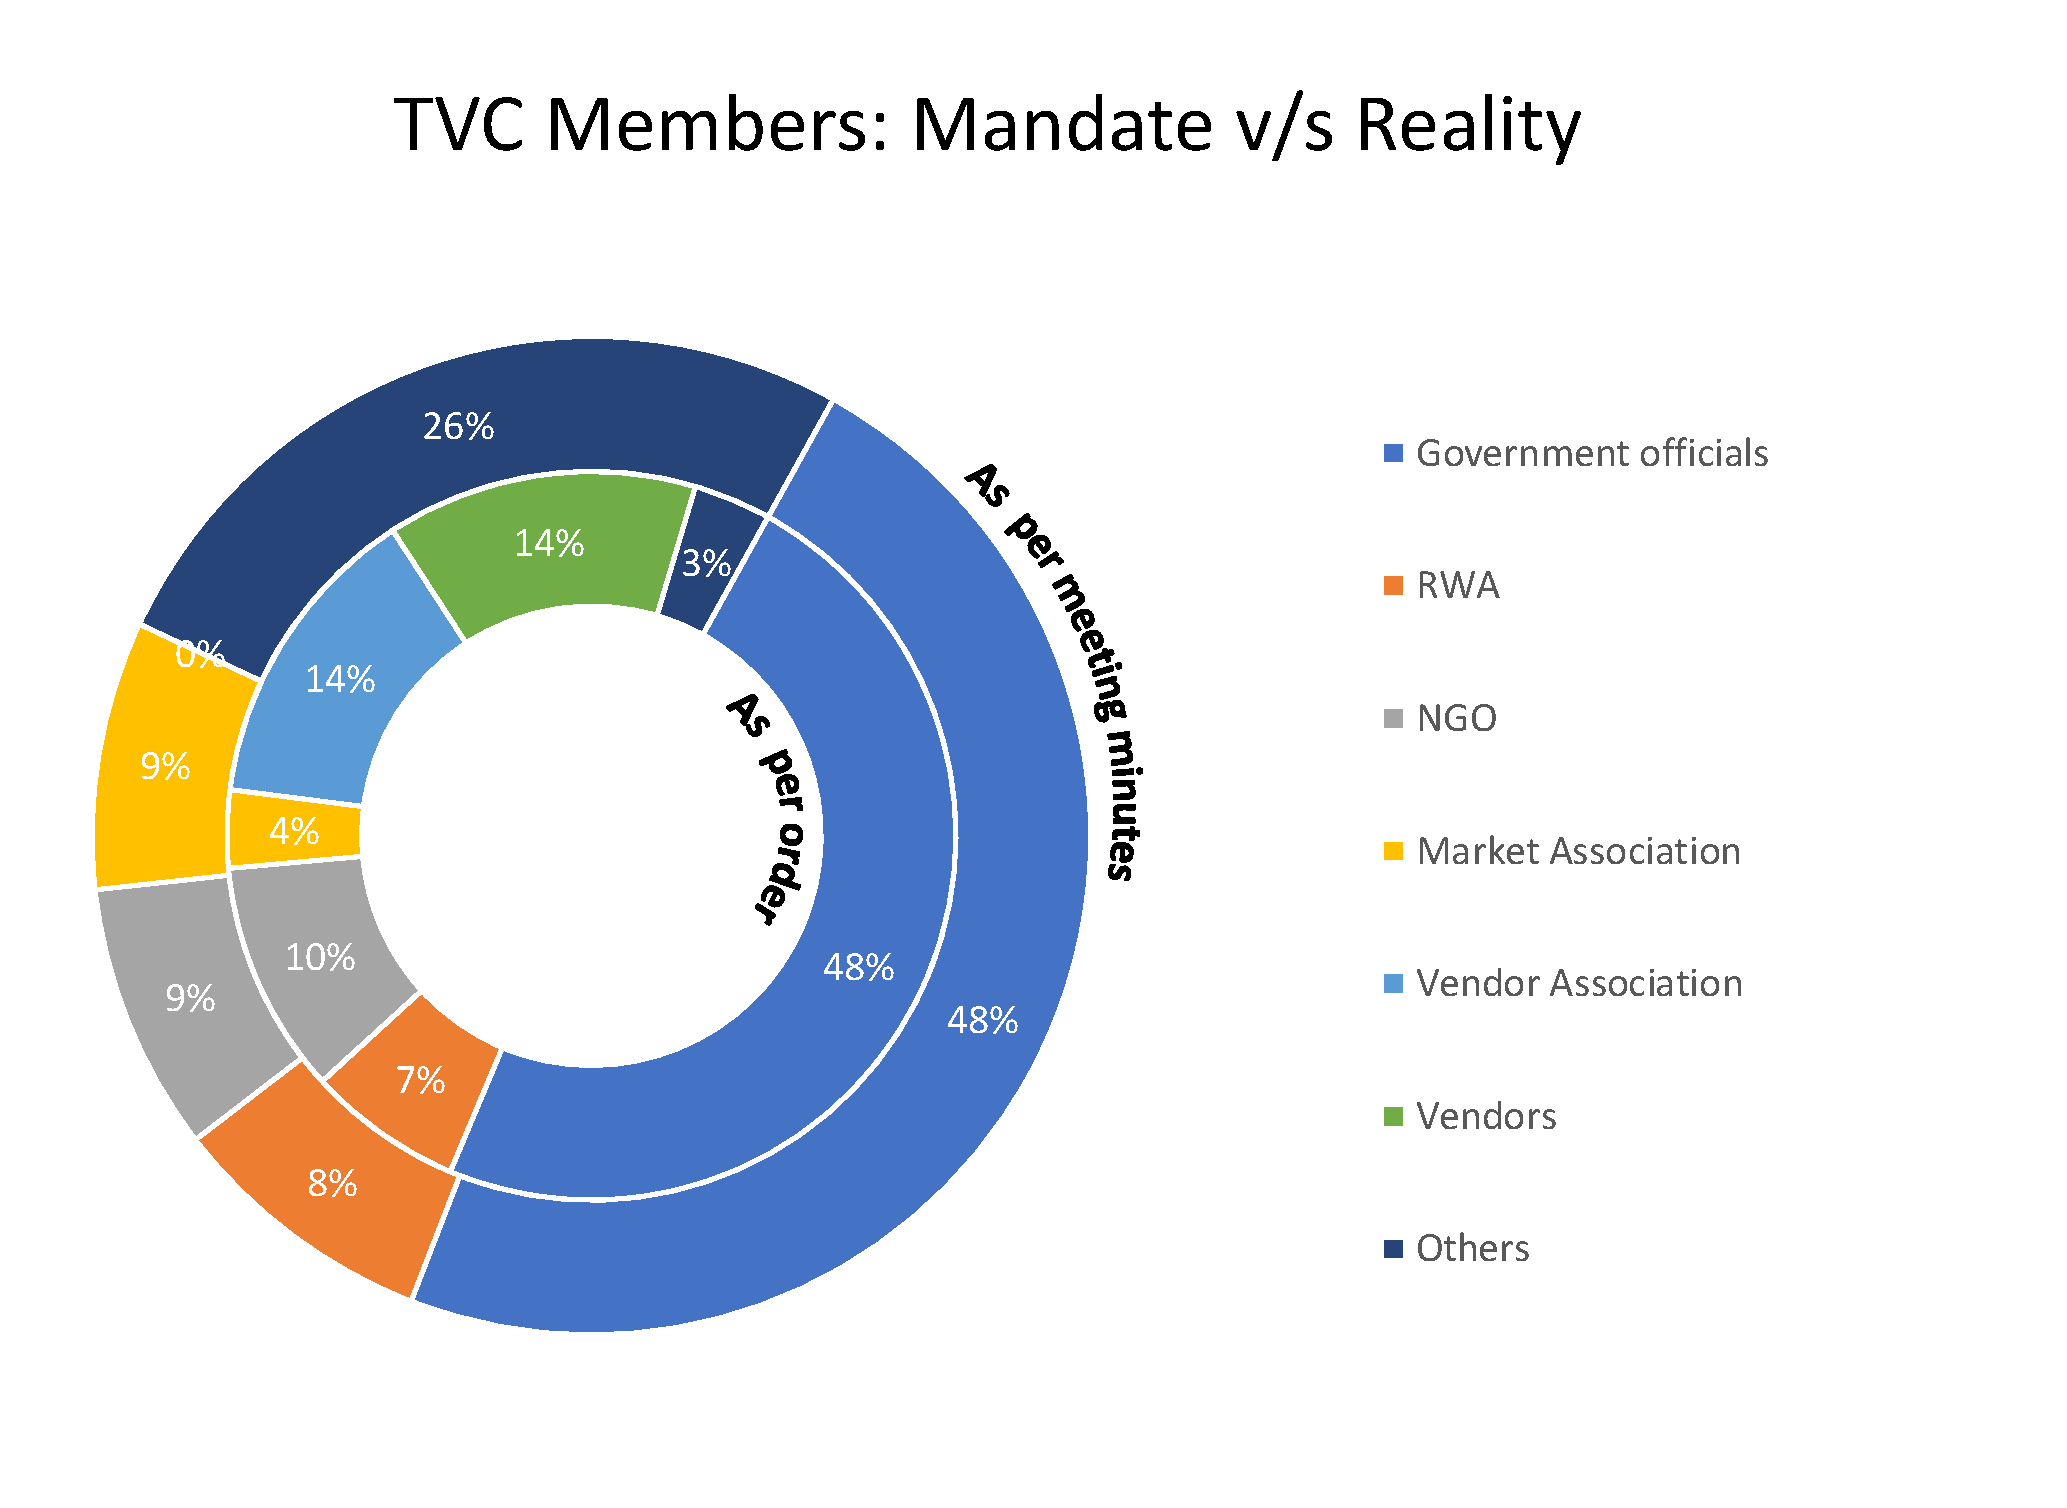
\includegraphics[width=0.6\textwidth]{mandatevsreality.pdf}
\end{wrapfigure}

The Act requires each TVC, headed by the Municipal Commissioner, to have at least 10\% representation from NGOs or community-based organisations and 40\% from vendors. Other members may include representation from the local authority, traffic or local police, banks, vendors, market associations and resident welfare associations (RWAs). Per the order from MCG dated 7 August 2018, vendors account for only 14\% of the total TVC strength of 29 members (Appendix \ref{sec: Appendix 6}).

Instead of being elected, as mandated by the Act and Haryana Street Vendor Rules 2017, the four vendor representatives were nominated. While the TVC more than fulfils its representation from the local authority, other government nominees, RWA and market welfare association, it falls 28\% short of the benchmark set in the Act on elected street vendor representation.

\subsection*{Mandate v/s Practice: Only 3 out of 17 Attendees Represented Vendors at the TVC Meeting, Resulting in Biased Decisions}
\addcontentsline{toc}{subsection}{Mandate v/s Practice: Only 3 out of 17 Attendees Represented Vendors at the TVC Meeting, Resulting in Biased Decisions}

The mandated list of TVC members of the local authority’s includes four vendors; however, the minutes of the meeting held on 21 August 2018 show zero representation from vendors (Appendix \ref{sec: List of TVC members}). The meeting had 23 signatories with no vendors, but the content of the minutes referred to the presence of three vendor representatives. When asked for a clarification, one of the vendor representatives explained that the discrepancy was due to the unwillingness of members to ratify minutes, given differences of opinion.

Separately, we also reached out to 15 of the 23 signatories to verify their presence at the meeting. Three denied being a part of any such meeting. One NGO member, on the condition of anonymity, mentioned that he was only present as he is “friends with the City Project Officer.”{\footnote{Respondent number 15, 21 and 22 from the list in Appendix 7 denied being a part of the TVC; one, being a representative from the market welfare association and second, the ad-hoc pradhan of Sector 14.}

\subsubsection*{Who Wins the Argument: Disagreement Between Government Officials and Vendors on Vending Sites}

The vendor representatives expressed disagreement with the TVC’s approach on withdrawal of two vending sites from Sector 14.

The meeting on 21 August 2018 was called to “take fair decision… regarding shifting of vending zones after hearing arguments of all concerned parties/stakeholders.” This was after three complaints by vendors to different authorities for reconsideration of the decision to withdraw sites. Out of the 17 members who voted on the decision, only 3 opposed. All three members were representatives of vendors. The minutes conclude by referring to the “democratically expressed views of the majority” and issued an order to shift vendors with “immediate effect.”

This example of the withdrawal of two sites from Sector 14 reflects how vendors may be overpowered easily in the absence of sufficient representation and a genuine will to formalise vendors. The effort here, it seems, is to obtain the majority to agree to a decision already decided. The meeting minutes repeatedly referred to the problems caused by vendors but were silent on the argument raised by vendors.

In Gurugram, the MCG has earmarked 49 vending zones—37 in September and 12 in October 2017. Some vendors registered to operate in  the earmarked vending zone  moved since the appointed vending zone was not in the vicinity of a residential area and experienced low levels of pedestrian footfall. Moving street vendors to the “off-street locations is relatively easy, but moving their customers to those locations is much more difficult. When customers fail to follow, the vendors have little choice but to return to the streets” \parencite{bromleypaper}.

These two examples raise questions on the willingness of municipality officials to include vendors in critical decisions. How are vending zones earmarked?\footnote{Meeting minutes of 21 August 2018 state: “as per approved layout plan of Haryana Urban Development Authority (HUDA), the site is earmarked for Parking and other is earmarked as Cycle Stand… prior to development of vending zones, permission was not obtained from Town and Country Planning Department to change use of sites as vending zone”.} In the case of disputes or conflicts, how are decisions made? Is there a structured channel of dispute resolution? How are the street vendors or their interests incorporated in such decisions?

\begin{wrapfigure}{r}{0.65\textwidth}
\centering
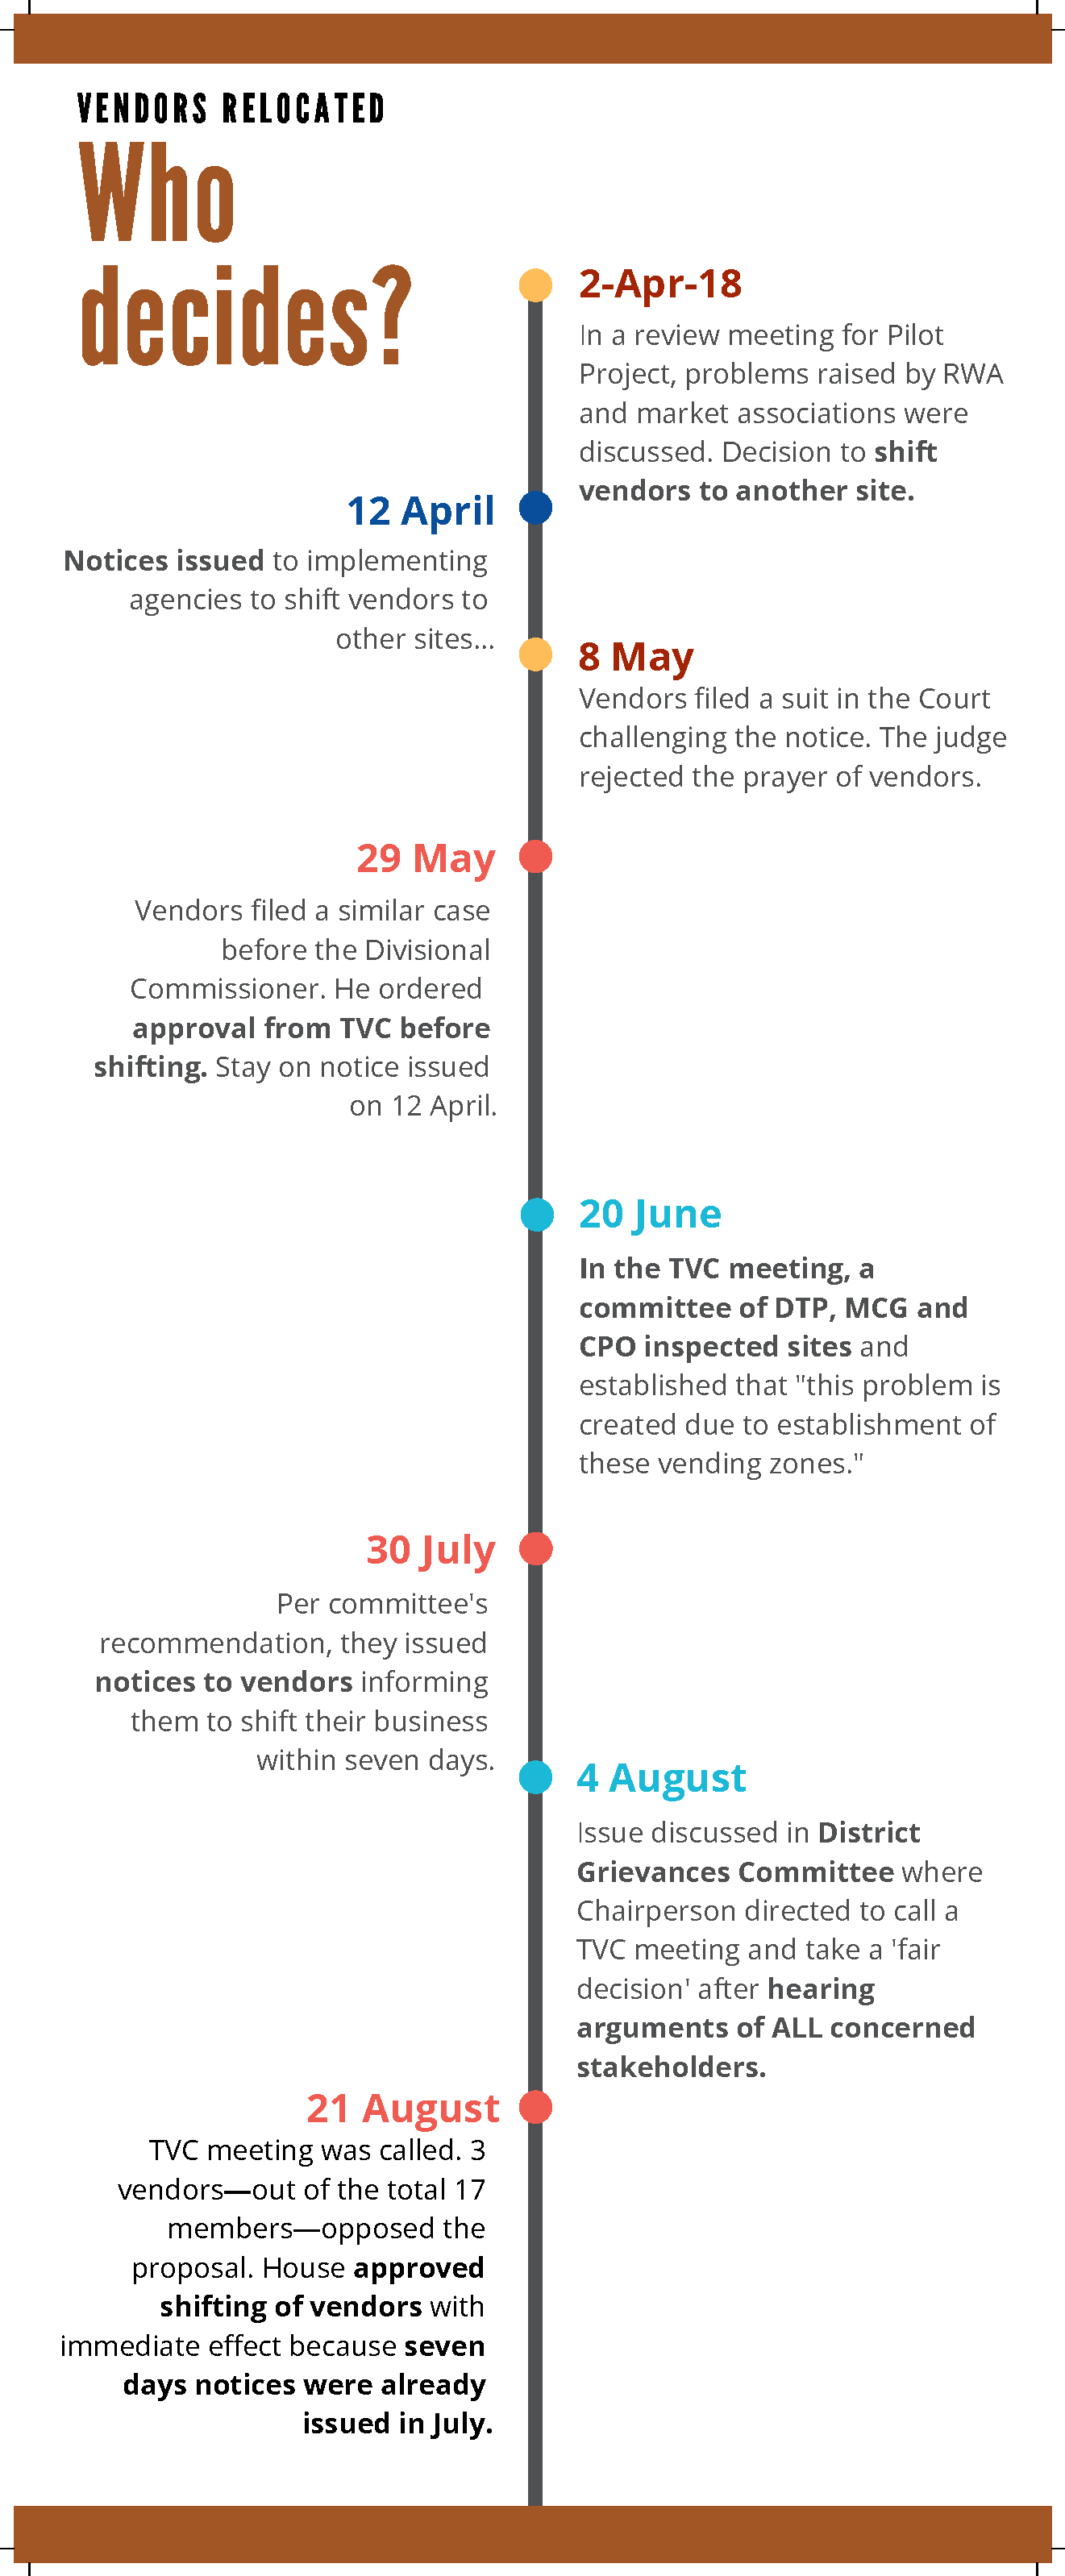
\includegraphics[height=1.15\textwidth]{WhoDecides.pdf}
\end{wrapfigure}

Although the Act opens channels and creates a super structure for negotiation between government and civil society, the devil lies in the detail. The suppression or protection of vendors will depend on the quality of regulations proposed by the local authority. The Act requires the plan for street vending to recognise the existing markets where buyers and sellers congregate. For any spatial planning exercise to be successful, it must take into consideration the commercial viability of vending sites. A thoughtful consideration of the existing patterns of vending and buy-in from vendors is necessary to ensure that the demarcation of zones does not become a futile exercise.

\subsection*{Contracting out TVC functions: Enabling or disabling Governance?}
\addcontentsline{toc}{subsection}{Contracting out TVC functions: Enabling or disabling Governance?}
The Act and the state government’s rules provide for the TVC to “temporarily associate itself with any person for their assistance or advice in carrying out provisions of the Act.” When MCG invited enterprises to participate in the pilot project, eight showed interest, and four were shortlisted between 2015 and 2016. The local body allotted sectors to the four shortlisted firms,  Spick and Span Services (SSSPL), Leo Mediacom, Egmac Capital and National Association of Street Vendors of India (NASVI), through draw of lots or a consensus.

Some of the core tasks delegated to the private firms include the following:
\begin{itemize}
\item Spatial planning taking into account natural markets, weekend markets, weekly haats, and night bazaars;
\item Demarcation of vending sites;
\item Design of carts to optimise space, keeping “aesthetics” into consideration;
\item Exhibit regulation and management of vendors;
\item Proposal for solid waste management;
\item Enumeration in allocated zones and;
\item Monitoring food adulteration and compliance with Food Safety and Standards Authority of India (FSSAI) norms.
\end{itemize}

Two years since the contract was signed, SSSPL has enumerated and registered vendors, and distributed carts in two out of seven allocated areas. In this section, we raise some questions on the enumeration exercise and fee imposed on vendors for the new carts.

\subsubsection*{Multiple Surveys, Multiple Identities?}
\addcontentsline{toc}{subsection}{Multiple Surveys, Multiple Identities?}

In Gurugram, the enumeration of vendors was first done in 2014. The exercise identified more than 14,000 vendors in all 35 wards. In 2016, the three private firms shortlisted for the regulation and management of vendors re-surveyed the sites to ensure that all vendors in the sectors allocated to them were enlisted. In 2018, the Haryana government started a new exercise that aspired to cover vendors of the whole state. \\

\begin{mdframed}[backgroundcolor=gray!20]
In one of our interviews with vendors, an unregistered vendor stated that in June 2018, the police authorities seized her cart goods on the grounds of it being a no-vending zone. She has been vending for 8 years at MG Road metro station; however, she was excluded in the enumeration exercise of 2014. Section 3.3 of the Act mandates that no street vendor shall be evicted or relocated till the enumeration exercise and issuance of a certificate to all vendors are complete. Moreover, the Act prohibits declaration of a no-vending zone before the completion of the enumeration and formulation of the street vending plan.

While she was allowed to reclaim her goods, she still can not vend for the fear of being evicted or harassed. In the absence of a one-stop grievance redressal committee, many vendors like her struggle to find the right platform to voice their concerns.
\end{mdframed}

The RTI response from government of Haryana, noted the identification of 18,670 vendors in Gurugram and the status of enumeration exercise as ‘ongoing’. By when will the survey be complete? What is the approach for conducting these surveys? How do these exercises by different enterprises guarantee identification of all vendors?

Streets are dynamic. Some vendors are stationary, some mobile. Even stationary vendors operate from multiple locations depending on the time of the year or day. Some operate full-time, some part time and others seasonally. Bromley (\cite*{bromleypaper}), writes, “The number of vendors rises and falls according to times of the year, week and day, responding to patterns of consumer demand and labor supply, to the cycles and fluctuations of the economy, and to levels of traffic congestion and official control.” The manner in which the local authority and other stakeholders accommodate the fluctuations is crucial for the exhaustive and accommodative registration of vendors.

\subsubsection*{Fees and Fines: What Does the Vendor Earn and Pay?}

\begin{wrapfigure}{l}{0.65\textwidth}
\centering
\includegraphics[width=0.65\textwidth]{"ggncart".png}
\end{wrapfigure}

The scheme for street vendors must provide for “the manner of collecting ...vending fees, maintenance charges and penalties for registration.”

Vendors in Gurugram, under the new policy, pay a one-time cart fee of Rs 85,000 to 1.5 lakh. The fee is decided based on the income of the vendor, and the nature of vending. It also varies depending on the the private enterprise in charge. The TVC meeting held in June 2016 discussed the possible ways of vendors to pay for the cart. The local authority officials refused to grant advertising rights to private enterprises; they were willing to provide carts free of cost to vendors, if such rights were accorded. Private parties alternatively offered to issue loans through banks/microcredit institutions to vendors in case they could not self-finance. Vendor representatives agreed stating that “street vendors are being harassed at multiple levels and they are willing to invest in anything which renders them recognition and security of tenure at a given location with the intent to safeguard their interest.”

The minutes did not give the rationale for the rejection of advertising rights. One of the key innovations of a similar public-private partnership in Bhubaneswar in 2006 was to obtain advertising firms to partly finance the carts.

In addition to the cart fee, vendors pay a monthly maintenance fee. SSSPL, for example, charges 1,500 (Appendix X). The MCG and the enterprise share the maintenance fee in the ratio of 1:2. The MCG generates an average revenue of Rs 10 to 12 lakhs annually from this.

The costs imposed on vendors and its impact are pertinent subjects but outside the scope of this study. Some of the questions for further research are as follows: Are vendors able to afford the “aesthetic” carts? How many vendors have been issued loans? What if vendors fail to replay? How are the funds generated through the collection of maintenance and other fees used?

\subsection*{No Mechanism for Dispute Redressal, Despite Piling Complaints}
\addcontentsline{toc}{subsection}{No Mechanism for Dispute Redressal, Despite Piling Complaints}

Section 20.1 of the Act requires the appropriate government to constitute a grievance redressal committee chaired by an ex-civil judge or judicial magistrate. In Gurugram, the City Project Officer personally attends to disputes.

As affirmed by the private enterprise, the lack of a grievance redressal committee makes it difficult for vendors to report harassment. The representative of the enterprise showed us a file full of complaints addressed to the MCG (Appendix \ref{sec: Appendix 9}. There is no information about the redressal status of these complaints.

In the TVC meeting held on 21 August 2018, the Assistant Commissioner of Police “assured that the police personnel will not harass the vendors unnecessarily and if any instance is noticed by the vendors/association, the same should be brought to the notice of DCP (HQ)/DCP (Traffic).” But during our interviews vendor association representatives were quick to point out that  vendors continue to be harassed and evicted—the police levied varying challan payments worth Rs 1,200 to 5,000 and the MCG charges Rs 5,000 to 10,000 for failure in maintaining cleanliness. The police officials also frequently seized their goods, reclaiming which was a tedious and lengthy process.

In the absence of a clear channel, how does the vendor solve the problems? Are these promises sufficient? What is the approach to curtailing evictions and other difficulties of vendors, until the formation of a grievance redressal committee? How will decisions be unbiased given that those vendors seek protection from—the police and municipality—are the ones who protect?

%===================CONCLUSIONS/RECOMMENDATIONS==================
\newpage
\section*{Conclusion}
\addcontentsline{toc}{section}{Conclusion}

Management of public space is a pressing problem in most space starved urban cities. India’s cities are no exception. “On its streets, India eats, works, sleeps, moves, celebrates and worships. The street is a stage that rarely sleeps,”wrote Arjun Appadurai in 1987 \parencite{naikpaper}. This study concerns itself with the key contender on Indian urban public space—the street vendor. Vendors are often accused of encroaching street, of depriving pedestrians of their walking space or for causing traffic jams. Municipalities, supported by the police officials, are quick to act on the complaints. The result is: harassment, demands for bribes, arbitrary confiscations, and physical abuse. Such actions, although undesirable, are rare when residents claim parking spots in front of their houses or when shopkeepers encroach land. From whom are public spaces being safeguarded and who is safeguarded?

Centre for Civil Society works to secure the rights of individual, especially informal workers, to life, liberty and property. The fight is not against a regulatory state but a state that is governed by arbitrary commands and the one that suppresses harmless livelihood opportunities. The Street Vendors Act 2014 was a landmark, in that after 50 years of judicial and regulatory clashes, it legitimise rights of street vendors and mandated states to create rules, schemes and local governance structures. What has changed?

There are three parts to the report: a look at the interpretation of the Act by the Higher Courts, a statistical capture of the progress by states in implementing the Act, and a case study of two urban cities to explore how the new Act is reshaping urban space management.

\subsection*{Role of Courts: No Protection in Times of Tardy Implementation}
Vendors have been a subject of several decisions ofthe Supreme Court and of numerous High courts in the last 50 years. We focused on judgements in the past year, that have come at a critical time of transition from multiple laws to one Act that overrides all existing laws.

Through our analysis of 57 court judgements, we find that eviction remains the most contested issue with 47 out of 57 cases dealing with what vendors considered unlawful evictions. Over half of these cases were decided against vendors. We find that several judgements undermine the spirit of the Act, particularly on two fronts. First, while the Act, for example, makes no distinction between a licensed and unlicensed street vendor, the High Court of Delhi took a different stand: only those vendors whose names were present in earlier lists prepared by the NDMC in 2007 or Supreme Court Committees could be protected under section 3(3).\footnote{ Section 3(3): No street vendor shall be evicted or, as the case may be, relocated till the survey specified under sub-section (1) has been completed and the certificate of vending is issued.} The High Courts of Calcutta and Kerala, in contrast, recognised the challenge of legal identity and either disallowed eviction or only allowed eviction where there was a case for “public interest.”  Second, High Courts have diluted section 33 that explicitly states that the Act overrides any law that has a bearing on vending rights. The High Court in Delhi, Madras and Kerala has allowed state laws to override the Act and authorities to evict vendors on the basis of this conflict. This is taxing for vendors who can only take legal recourse for challenging the arbitrary use of power by local authorities. Encouraging evictions without extending any interim protection or relocation reinforce the existing bias against vendors’ ‘right to the city.’

\subsection*{Progress by State Governments: Slow to Show}
Monitoring state progress on compliance helps ensure we have the systems in place necessary to bring reform. In 2018, we extended our work from 2017 on measuring absolute and relative progress on state compliance based on self-reported data. Out of the 30 states analysed, we find that 11 are yet to notify the scheme—the statutory deadline for which was October 2014. Of the 7,263 towns from 30 states, over 65\% are yet to form a TVC. Only 58\% of these TVCs have vendor representatives. Any functions performed by a TVC without vendor representatives may be legally untenable since they violate the mandate of the Act.

To measure relative compliance, we give each state a score based on their performance on 11 steps encompassing notification of rules and schemes, formation of TVCs with vendor representation, enumeration of vendors, issuance of vending certificates, assignment of office space, demarcation of vending zones, and publication of charter and vending plans. We have assigned a higher weightage to rule-making and creation of institutions—without which implementation can be and has been questioned in the Court. Tamil Nadu, Mizoram, Chandigarh and Rajasthan have performed the best. Nagaland, West Bengal, Sikkim, Karnataka and Manipur lag far behind. West Bengal has 3 TVCs for 239 towns and Nagaland has 2 TVCs for 11 towns. Both states have only implemented two out of 11 steps of implemented.

\subsection*{Up Close: New Structures Attempt to Suppress}
While the index—based on self-reported data—gives a bird’s eye view of the extent and depth of compliance, it does not capture state idiosyncrasies or the gap between claimed and actual implementation. We studied two TVCs, a small but critical unit of governance, in the populous city, Delhi and the its satellite town, Gurugram.

In Gurugram, the MCG mandated list of TVC members had only 14\% (4/29) vendor representation as opposed to 40\% required by the Act. Vendor representatives present in actual meetings were different (and fewer)than those in the proposed list. Analysis of meeting minutes show that actions were taken against vendor demands, and this was after vendors raised complaints with three different authorities. The minutes had no space for the ‘voice’ of vendors—we know that vendors objected, the reasons for their objection were not recorded.

Gurugram is unique in its approach to contract selected functions of the TVC to private firms, raising questions on state capacity to use in-house resourced to enumerate and certify vendors.
In Delhi, … (yet to add)

In SumThe Act has the potential to redefine historically ambivalent vendors’ rights to  city’s public spaces. Success, however, rests on the capacity and willingness of vendors and state administrators to cooperate. In absence of penalties for non-compliance, progress at the state level has been sluggish. As the rules and schemes are being notified, the next step is to evaluate the details: whether the new regulatory tools are used to prioritise or delegitimize vendors’ rights. Unless we establish rule of law for the use of public space, mechanisms to redress grievances and build the capacity of vendors to negotiate with administrators as they balance the many citizens rights to livelihood, safety, essential urban services, and public commons—the street will continue to seed conflict.


%===================BIBLIOGRAPHY====================================
\newpage
\section*{Bibliography}
\addcontentsline{toc}{section}{Bibliography}
\printbibliography[heading=none]

%===================APPENDICES======================================
%Appendix 1
\newpage
            \begin{landscape}
\section*{Appendix 1: References for Legal Analysis}
\addcontentsline{toc}{section}{Appendix 1: References for Legal Analysis}
\label{sec: Appendix 1}
            \scriptsize
              \rowcolors{3}{gray!25}{white}
            \begin{longtable}{>{\raggedright}p{1.5cm}>{\raggedright}p{2.5cm}>{\raggedright}p{1.3cm}>{\raggedright}p{1.5cm}>{\raggedright}p{1.1cm}>{\raggedright}p{1.2cm}>{\raggedright}p{1cm}>{\raggedright}p{1.8cm}>{\raggedright}p{1.3cm}>{\raggedright}p{4.45cm}>{\raggedright\arraybackslash}p{1.2cm}}
          
            \caption{Street Vendor Case Data}\\

Case Citation &
Case Title &
Case No. &
Court &
State &
Date of \\ Judgement &
Relevant \\ (Y/N) &
Issue &
Outcome &
Decisions/Rule Laid Down &
Significance (1-5) \footnotemark \\
\midrule
\endfirsthead
%\rotatebox[origin=c]{90}
Case Citation &
Case Title &
Case No. &
Court &
State &
Date of \\ Judgement &
Relevant \\ (Y/N) &
Issue &
Outcome &
Decisions/Rule Laid Down &
Significance (1-5) \\
\midrule
\endhead
\bottomrule
\endfoot
\bottomrule
\endlastfoot
\footnotetext{Significance indicated the likelihood of a case to be quoted and cited in subsequent decisions.}

MANU/TN/10\\57/2018 & A.T. Mhammed Ismail and Ors. v The Commissioner Greater Chennai Corporation and Ors & W.P. Nos. 4171 and 4172 of 2018 & High Court of Madras & Tamil Nadu & 2/26/2018 & Y & Eviction & Deferred  & When statute contemplates issuance of certificate, and right to carry on business of street vending in accordance with the terms and conditions mentioned in the certificate of vending, and when a representation is made by the street vendors, it is the duty of the competent authority to consider such representation and pass appropriate orders. & 2  \\

MANU/KE/20\\75/2018 & Abbas V. and Ors v State of Kerala and Ors.  & WP(C) No. 25239 of 2018 & High Court of Kerala & Kerala & 7/26/2018  & Y & Eviction; Due Process; Relocation; Legislative Overlap  & Deferred & Competant authority to consider applications after hearing the petitioners without much delay, preferably within two months. (approach the highway authority u/s 4 of the kerela highway protection act to seek permission for doing business. & 2 \\

MANU/TN/54\\75/2018 & D.S.Sundar v The Special Commissioner for Handicapped and Ors. & WPC 16054 of 2013 & High Court of Madras & Tamil Nadu & 9/20/2018 & Y & Eviction; Definition of Street Vendor (whether a bunk owner is a street vendor) & Deferred & Petitioners to approach the TVC to consider all other aspects including public utility and other practical difficulties. & 2 \\

2017 SCC ONLINE P\&H4106 & Deepu Sharma v State of Punjab & CWP 5816 of 2015 (O\&M) & High Court of Punjab \& Haryana & Punjab & 9/7/2017 & Y & Harassment; Eviction; Survey & Directions & Petitioners to approach the TVC to consider all other aspects including public utility and other practical difficulties. & 2 \\

MANU/DE/23\\11/2018 & Delhi Pradesh Rehri Patri Khomcha Hawkers Union and Ors. v South Delhi Municipal Corporation and Ors. & W.P. (C) 6672-6673/2018 & High Court of Delhi & Delhi &7/3/2017  & Y & Elections; Display the zone-wise voter list, vote-applicant list etc. & Partially dismissed & - \quotes{ ...In case the Petitioners were aggrieved by the procedure which was being followed by
the Corporations, they should have approached this Court at the earliest point of
time. \[...\] - We are also of the view that in case the objections are invited, at this stage it
would not only result in elections being postponed but would also be in violation of
the orders passed by the Supreme Court of India.} & 3 \\

2018 SCC ONLINE DEL 8251 & G.Raju v North Delhi Municipal Corporation & WP (C) 2588 of 2018 & High Court of Delhi &  Delhi & 3/19/2018 & Y & Eviction & Deferred & Directions:

(i)The Petitioner to approach TVC as and when constituted with all the supporting documents.

(ii) TVC to consider the documents in accordance with the law expeditiously.

(iii) Merely because the petitioner is not found vending at the site when the survey is conducted  that by it self would not be a ground alone to reject his case. & 1 \\

MANU/KE/21\\26/2018 & K.H Abdul Rahman v District Industries Centre and Ors. & WP(C) 3108/2018 & High Court of Kerala &  Kerala & 8/10/2018 & Y & Eviction; CoV & Deferred  & Deferred to TVC & 1 \\

2017 SCC ONLINE KER 9727 & Karutha Lakshmi v District Collector, Civil Station, Kannur & WPC 28290/2016 & High Court of Kerala & Kerala & 3/2/2017 & Y & Due Process; Eviction & Deferred  & An opportunity of being heard to be provided to the Petitioner & 2 \\

2017 SCC ONLINE MAD 31753 & Marimuthu v Corporation of Chennai & WP 26333/2017 & High Court of Madras & Tamil Nadu & 10/12/2017 & Y & Eviction ; CoV & Deferred  & Representation/request to be considered by TVC within a period of one month &  1 \\

2018 SCC ONLINE DEL 6476 & Mukesh Kumar v New Delhi Municipal Council and Anr & WP(C) 61/2018 & High Court of Delhi & Delhi & 1/5/2018 & Y & Eviction & Deferred  & 1. The Petitioner would approach the TVC as and when it is constituted with all the supporting documents.

2. TVC will consider the case of the petitioner in accordance with law and expeditiously after considering all the material on record.

3. Merely because the Petitioner is not found vending at the site when the survey is conducted, that would not be a ground alone to reject his case. & 1 \\

2017 SCC ONLINE KER 34700 & Murali vs State of Kerala & WP(C) 32001/2017 & High Court of Kerala & Kerela & 11/2/2017 & Y & Eviction & Deferred  & The Petitioner to show cause; no evicton until a final decision is taken & 1 \\

2018 SCC ONLINE MAD 1392 & N. Murugan v Joint Commissioner  & WP (MD) 10584 of 2018 & High Court of Madras & Tamil Nadu & 5/3/2018 & Y & Fee-collection Right to be auctioned & Dismissed & \quotes{*Public auction cum tender notification (right to collect fees from the street vendors) for auctioning the collection right challenged

* Grounds for challenge: a representation submitted for renewal of his right, he being the successful bidder for the previous year

* Representation already rejected by the government

* Writ dismissed with liberty to challenge the order rejecting the request of the petitioner.} & 2\\

2018 SCC ONLINE DEL 6813 & Nanni Bai Ahirwar v New Delhi Municipal Council and Anr & WP(C) 673/2018 & High Court of Delhi & Delhi & 1/23/2018 & Y & Permission for change of trade & Deferred  & \quotes{1. The Petitioner would approach the TVC as and when it is constituted with all the supporting documents.

2. TVC will consider the case of the petitioner in accordance with law and expeditiously after considering all the material on record.

3. Merely because the petitioner is not found vending at the site when the survey is conducted , that by it self would not be a ground alone to reject his case.} & 1 \\

2017 SCC ONLINE MAD 27698 & P.Arun Kumar v State Commisioner for Differently Abled   & WP 19858 of 2017 & High Court of Madras & Tamil Nadu & 9/20/2017 & Y & Eviction; definition of street vendor & Deferred  & \quotes{1. Quoted WPC 18677 of 2014, order dated 3.09.2015: "street vendor" includes one selling from a temporary built up structure

2. TVC yet to be constituted: Respondent 2-4 shall consider the claim of the petitioner re: applicability of SVA 2014 within 12 weeks; until then bunkshop not to be disturbed} & 2\\

2017 SCC ONLINE MAD 2159 & P. Rajam v Corporation of Chennai & WP 22515/2014 & High Court of Madras & Tamil Nadu & 6/7/2017 & Y & CoV & Deferred & Petitioner may move an application to TVC within two weeks & 1\\

MANU/SCOR\\/01337/2017 & Paguthi Small Viyaparigal Sangam and State of Tamil Nadu and ors. & Petitions for Special Leave to Appeal C Nos. 857/2017 & Supreme Court of India & India & 1/11/2017 & Y & Eviction & Deferred  &  & 1\\

MANU/TN/55\\38/2018 & Palani v Government of Tamil Nadu and Ors &WP 2232/2018 and WMP 2730/2018 & High Court of Madras & Tamil Nadu & 9/18/2018 & Y & Vending zone; Relocation; Implementation & Directions & Noted the steps for implementation already being taken by the Government authorities to implement the Act. & 2 \\

2017 SCC ONLINE MAD 30457 & Ramanathan Theru Usman Road Kizhaku Paguthi Small Viyaparigal Sangam v A.K. Vishwanathan & Cont. Pet. No. 952/2017 & High Court of Madras & Tamil Nadu & 10/4/2017 & Y & Contempt; Eviction & Directions & Police not to cause any disturbance to existing street vendors until a decision is taken by vending committee; Police prevented only new entrants so as to maintain free flow of traffic and avoid any public inconvenience & 3 \\

MANU/RH/02\\12/2017 & Ravindra Singh and Ors.v State of Rajasthan and Ors & \quotes{SB CWP 17763, 8415/2016, 10451, 1026/2015, 377, 5019 and 4471/2017} & High Court of Rajasthan & Rajasthan & 4/6/2017 & Y & Eviction & Directions & \quotes{(Para 11) Till the directions aforesaid are completed, the existing vendors would not be disturbed in the light of sub-section 3 of Section 3 of the Act of 2014, however, directions would not apply to the area which are otherwise covered by any other judgment of this Court directing the Municipal Corporation not to allow vending in that area.} & 3 \\

2017 SCC ONLINE KER 13854 & Sabu M.J v Corporation of Kochi & WP(C)10547/2017 & High Court of Kerala & Kerala & 3/30/2017 & Y & Eviction & Deferred &Direction to the Deputy Mayor to consider the petitioner's representation in accordance with law within two weeks; no eviction without relocation & 3 \\

MANU/KE/20\\97/2018 & Saji Joy v The Executive Engineer, PWD NH Division and Ors & W.P.(C)18356, 23827/2018 & High Court of Kerala & Kerala & 8/7/2018 & Y & Eviction; Relocation; Legislative Overlap & Deferred & Competant Authority to consider applications after hearing the Petitioners without much delay. & 2\\

MANU/UP/12\\73/2018 & Satender Kumar and Ors v State of U.P. and Ors & Writ-C 8602/2018 & High Court of Allahabad & Uttar Pradesh & 3/7/2018 & Y & Eviction; Implementation & Directions & \quotes{The authority shall undertake and complete the survey as contemplated under the 2014 Act and proceed to identify and create vending zones in accordance with the statutory provisions. As and when the vending zones are created, it shall be open for the petitioners to seek their registration as street vendors under the Act aforementioned and apply for allotment.} & 3\\

MANU/SCOR\\/17149/2018 & Self Employed Welfare Association v The State Commissioner for Differently Abled \& Ors & SLP C 9857/2018 & Supreme Court of India & India & 5/18/2018 & Y & Survey; Implementation & Directions & Survey to be conducted within a month & 2 \\

2017 SCC ONLINE KER 12837 & Shamsu C v Corporation of Cochi & WP(C) 25597/2013 & High Court of Kerala & Kerala & 3/24/2017 & Y & Eviction; Relocation; Entitlement & Deferred & For factual determination of the question of entitlement of the petitioner to occupy the bunk shop, an opportunity to be provided to the petitioner to put forth his claim before the corporation of kochi or TVC if already constituted  & 3\\

2017 SCC ONLINE DEL 8202 & Sheetal Prasad Gupta v New Delhi Municipal Council & WP(C)11592/2016 & High Court of Delhi & Delhi & 4/25/2017 & Y & Eviction; Relocation; definition & Directions; consent decree & Name of the petitioners find mentioned in the list of 628 vendors prepared by the NDMC; hence to be relocated & 2\\

2018 SCC ONLINE DEL 8150 & Sita Rawat v South Delhi Municipal Corporation & WP(C) 1293/2018 & High Court of Delhi & Delhi & 3/7/2018 & Y & Eviction & Deferred & \quotes{1. The Petitioner would approach the TVC as and when it is constituted with all the supporting documents.

2. TVC will consider the case of the petitioner in accordance with law and expeditiously after considering all the material on record.

3. Merely because the Petitioner is not found vending at the site when the survey is conducted , that by it self would not be a ground alone to reject his case.

4. Rules are notified.} & 1\\

MANU/KE/17\\24/2018 & Sudheesh T.S v State of Kerela and Ors & WP(C) 17792/2018 & High Court of Kerala & Kerela & 7/10/2018 & Y & Eviction ; Relocation; Legislative Overlap & Deferred & Competent Authority to consider applications after hearing the Petitioners without much delay. &  \\

2017 SCC ONLINE BOM 571 & Thane Zilla (Maharashtra) Hawkers Union v State of Maharastra and Ors & WP (ST) 4622/2017 & High Court of Bombay & Maharash tra & 3/6/2017 & Y & TVC constituted without street vendor representation & Directions & \quotes{1) Local authorities to comeback with a statement as to how they intent to remove the anamoly created;

2) Local authority to keep 8 vacancies unfilled in the TVC can proceed with the other 12 members.} & 3 \\

MANU/KE/17\\22/2018 & V.Prabhakaran and ors v National Highway Authority, Kozhikode and Ors & WP(C) 17377/2018 & High Court of Kerala & Kerela & 7/17/2018 & Y & Eviction; Relocation; Legislative Overlap & Deferred & Competant authority to consider applications after hearing the petitioners without much delay. & 2\\

MANU/DE/20\\90/2018 & Vijay Kumar Sahu and Ors v Govt. of NCT and Ors & W.P.(C) 7785/2017 & High Court of Delhi & Delhi & 5/29/2018 & Y & Eviction & Deferred & Rules notified; public notice issued for inviting applications with supporting documents; the Petitioner to approach the TVC as and when it is functional; TVC to consider the case. & 2\\

2018 SCC ONLINE DEL 7578 & Vijender v South Delhi Municipal Corporation & WP (C) 2291/2017 & High Court of Delhi & Delhi & 2/12/2018 & Y & Eviction & Deferred & Adjourned the matter for a period of three months to enable theTVC to become functional. & 2 \\

2017 SCC ONLINE DEL 11779 & Virender v South Delhi Municipal Corporation & WP(C) 11552/2016 & High Court of Delhi & Delhi & 10/25/2017 & Y & Definition- Street Vendor; Eviction & Partially dismissed; consent decree & No-vending zone as decided prior to the Act to be continued; Act is applicable only to \quotes{regular street vendors}. No relief to be granted to petitioner 1 to 9 who are not regular street vendors. & 2 \\

\end{longtable}
\end{landscape}


%Appendix 2
\newpage
\section*{Appendix 2: Formula Used to Calculate the Index}
\addcontentsline{toc}{section}{Appendix 2: Formula Used to Calculate the Index}
\label{sec: Appendix 2}
Formula used to calculate the index:
\begin{align*}
SVC_n &= \sum_{i = 1}^{i = n} \alpha_i V_i
\end{align*}

where $n$ is the state for which the score is being calculated, $\alpha_i$ is the weight accorded to the variable $V_i$ for the $i$th attribute.

The focus of the index is first on rule-making and establishment of institutions and bodies, for example, TVCs and Grievance Redressal Committees and only after on implementation steps. Without institutions, as mandated by the Act, implementation can be challenged.

The weights indicate the importance ascribed to each step. Higher weight is ascribed to steps that form the basis of all other steps, such as notification of rules and schemes. Without rules and schemes, the process followed to form TVCs or to conduct surveys might be questioned.

Similarly, actions of TVC without vendor representatives may be challenged in the court as the Act mandates TVC to have 40\% vendor representation from vendors.

%Table 7: Variables and Weights Used for Calculation of State Score
\begin{longtable}[l]{>{\raggedright}p{1.5cm}>{\raggedright}p{6cm}>{\raggedright}p{2.5cm}>{\raggedright\arraybackslash}p{4cm}}
  \caption{Variables and Weights Used for Calculation of State Score}\\
    \toprule
$V_i$ & Variable & Weight $(\alpha_i)$ & Variable into Weight \\
\midrule
\endfirsthead
$V_i$ & Variable & Weight $(\alpha_i)$ & Variable into Weight \\
\midrule
\endhead
\bottomrule
\endfoot
\bottomrule
\endlastfoot
$V_1$ & Whether the state government has notified the rules for implementing the Act (1 if drafted; 0 if not drafted) & 13 & $13 * V_1$\\
$V_2$ & Whether the state government has notified the scheme for implementing the Act (1 if drafted; 0 if not drafted) & 13 & $13 * V_2$\\
$V_3$ & Proportion of towns with a Grievance Redressal Committee & 11 & $11 * V_3$\\
$V_4$ & Proportion of towns with TVC & 11 & $11 * V_4$\\
$V_5$ & Proportion of TVCs with \textbf{vendor representatives} & 10 & $10 * V_5$\\
$V_6$ & Proportion of TVCs that have \textbf{conducted survey} & 10 & $10 * V_6$\\
$V_7$ & Proportion of TVCs that have \textbf{issued identity cards to more than 75\% of identified vendors} & 8 & $8 * V_7$\\
$V_8$ & Proportion of TVCs that have \textbf{earmarked vending zones} & 7 & $7 * V_8$\\
$V_9$ & Proportion of TVCs that have \textbf{a vending plan} & 7 & $7 * V_9$\\
$V_{10}$ & Proportion of TVCs that have \textbf{published a charter} & 6 & $6 * V_{10}$\\
$V_{11}$ & Proportion of TVCs that have \textbf{assigned office space} & 4 & $4 * V_{11}$\\
\midrule
& & 100 & $\sum_{i = 1}^{i = n} \alpha_i V_i$\\
\end{longtable}

%Appendix 3
\newpage
\section*{Appendix 3: Questionnaire for SV Act Implementation}
\addcontentsline{toc}{section}{Appendix 3: Questionnaire for SV Act Implementation}
\label{sec: Appendix 5}


\begin{mdframed}[backgroundcolor=gray!20]
\textbf{Module A: Basic information}

A1. Name of the respondent: 

A2. Gender: M/F/Other

A3. Designation in committee:


\textbf{Module B: Constitution of a Town Vending Committee}

B1. How many TVCs are there in Gurugram currently?

B2. When was this TVC formed? (mm/yyyy)

B3. How many members are there on the committee?

B4. What is your role in the committee? (Specify organisation where necessary)

\begin{enumerate}[nosep]
\item Municipal commissioner
\item Local body official
\item Traffic Police official
\item Local Police official
\item Market/Trader Association:
\item Street Vendors Association:
\item NGO/community based organization member:
\item RWA member
\item Street vendors
\item Others, please specify
\end{enumerate}

Ask B5-6 if answer to B4 is Municipal commissioner

B5. Were the rules and scheme formed prior to the formation of the TVC? (ask for specific dates)

B6. Who is the Chairperson of the town vending committee of each ward/zone?

B7. Since when have you been a part of this TVC?

B8. How did you become a part of the committee?
\begin{enumerate}[nosep]
\item Nomination
\item Election
\item Others, please specify
\end{enumerate}

B9. What are your responsibilities in the committee? (Enlist top five)

B10. What is your interest as a part of this committee? (Pick top three concerns)
\begin{enumerate}[nosep]
\item Voice resident concerns
\item Voice vendor interests and challenges
\item Represent government interests
\item Voice concerns of existing natural markets
\item Reduce street vendors in the area
\item Increase street vendors in the area
\item Ensure cleanliness
\item Prevent traffic congestion
\item To attend the meetings
\item Others, please specify
\end{enumerate}

\textbf{Module C: Operation and Activities}

C1. How many meetings of the TVC were held in the last 6 months?

C2. Where and how are minutes of it recorded?

C3. Is attendance marked? (Ask for records of the last 3 dates of meetings and MOM)

C4. Is there a designated office space for the Town Vending Committee? (Skip C3 if the answer is no)

C5. Where is it located?

C6. According to the rules, what activities have been completed by your TVC? (Use options to give examples)
\begin{enumerate}[nosep]
\item Election for electing street vendors
\item Formed Grievance Redressal Committee
\item Identified street vendors
\item Identified vending zones
\item Issued ID cards and certificate of vending
\item Drafted plan of vocation for street vendors
\end{enumerate}

C7. What is the order followed to complete the above activities?

C8: Has the committee marked vending zones? (Skip C5 if the answer is no)

C9. What factors are considered to mark vending zones? (Use options to give examples)
(By natural markets, we mean: a market where sellers and buyers have traditionally congregated for the sale and purchase of products or services)
\begin{enumerate}[nosep]
\item Traffic
\item Locations preferred by the public
\item Existing residents
\item Existing natural markets
\item Preference of vendors
\item Others:
\end{enumerate}

C10. How do you decide the holding capacity of the area?

C11. Which body looks at vendor grievances?
\begin{enumerate}[nosep]
\item Grievance redressal committee
\item TVC
\item Local authority
\item Others
\end{enumerate}

C12. What is the process for filing grievances?

C13.  For which of the following does the committee maintain records?
\begin{enumerate}[nosep]
\item Total numbers of street vendors identified
\item Vending zones
\item Registered vendors
\item Licenses issued
\item Location of vendors
\item Revenue generated through fee collected
\item Challan issued
\item Fine imposed
\item No, we do not maintain records
\item Others
\end{enumerate}

C14. How are the records maintained? (Request documents)
\begin{enumerate}[nosep]
\item Electronically
\item Manually
\end{enumerate}


C15. What are the sources of revenue for the committee?
\begin{enumerate}[nosep]
\item Funded by the government
\item Vending fee
\item Challans/fines
\item Others
\end{enumerate}


C16. What is the amount for the following charges collected from the vendors:
\begin{enumerate}[nosep]
\item Vending fee
\item Maintenance fee
\item Others
\end{enumerate}


C17. Is the vending/maintenance fee uniform in all vending zones?


C18. What is the procedure in case a vendor can’t pay the vending/maintenance fee?


C19. What fines/challans are applicable to the vendors, in case of non-compliance:
\begin{enumerate}[nosep]
\item Penalty fee
\item Challans
\item Others
\end{enumerate}

\textbf{Module D: Street Vendors’ Representation and Election}

(The Act mandates 40\% of any TVC to be street vendors with due representation to SC, ST and other backward classes)

D1. Does the TVC have street vendors’ representatives? If no, why not?

Ask D2-D8 only if the answer to D1 is yes

D2. How many street vendors’ representatives does the TVC have?

D3. If yes, how were the members appointed?
\begin{enumerate}[nosep]
\item Nomination
\item Election
\item Lottery system
\item Other, please specify
\end{enumerate}

Ask D4-D9 only if the answer to D2 is ‘election’

D4. How were the elections announced?

D5. Which authority/officer was responsible to conduct the elections?
\begin{enumerate}[nosep]
\item Municipal Corporation
\item Municipal Council/Committee
\item Planning Authority
\item Other, please specify
\end{enumerate}

D6. What is the eligibility criteria to vote?

D7. How are the zones decided for elections?

       (subjectivity of documents that makes them eligible to vote, zones where elections are held,
       zones and vendors left out)

D8. What is the basis of shortlisting the contesting candidates?
\begin{enumerate}[nosep]
\item Compliance of mandatory provisions as under Act and Rules
\item Submission of authentic mandatory documents
\item Missing signature on declaration form for nomination
\item Other, please specify
\end{enumerate}

D9. How are the names of elected members notified?
\begin{enumerate}[nosep]
\item Website
\item ULB office
\item Other, please specify
\end{enumerate}
\end{mdframed}

\begin{mdframed}[backgroundcolor=gray!20]
\subsection*{Private Enterprise hired for Act Implementation under Pilot Project}

\textbf{Module A: Basic information}

A1. Name of the respondent:

A2. Organization:

A3. Designation:

A4. What does your enterprise do?

\textbf{Module B: Their role under SV Project}

B1. How was your agency selected for this project?

B2. What are the tasks you are accountable for, as part of the pilot of SV project?

B3. Which zones are your responsible for? (Enlist all)

B4. How often does your agency report to the MCG?

B5. What is the amount for the following charges collected from the vendors:
\begin{enumerate}[nosep]
\item Convenience fee
\item Cart fee
\item Maintenance fee
\item Others
\end{enumerate}

B6.  What is the mode of fee collection?

B7. What is the process followed for fee collection?

B8. How are revenues shared with the MCG?

B9. Do you assist the MCG in registration of vendors?

B10. What is the process followed to register vendors?

B11. Do you distribute any IDs to the vendors? (Share copy)

B12. Do you have a role in spatial mapping of zones under the project?

B13. Enforcement and regulation is sole responsibility of the firm. What does this entail?

B14. What factors are considered to inspect vendors?
\begin{enumerate}[nosep]
\item Adulteration (FSSAI norms), in case of food vendors
\item Sanitation and hygiene
\item Others
\end{enumerate}

B15. Does any team from MCG visit the sites under your jurisdiction?

B16. What is the frequency of their visits?

B17.  For which of the following does your agency maintain records?
\begin{enumerate}[nosep]
\item Total numbers of street vendors identified
\item Vending zones
\item Registered vendors
\item ID cards issued
\item Revenue generated through fee collected
\item Others
\end{enumerate}

B18. What are the challenges/risks associated with this pilot project?

\textbf{Module C: Town Vending Committee}

C1. Are you aware of the Street Vendors Act 2014?

C2. Are you aware about the Town Vending Committee (TVC)?

C3. Are you a part of the TVC? (Skip B4-B16 if the answer is no)

C5. What is your role in the committee? (Specify organisation where necessary)

C6. Since when have you been a part of this TVC?

C7. How many meetings of the TVC were held in the last 6 months?

C8. Does the TVC have street vendors’ representatives? (Skip B15 if the answer is no)

C9. How many street vendors’ representatives does the TVC have?

C10. Which body looks at vendor grievances?
\begin{enumerate}[nosep]
\item Grievance redressal committee
\item TVC
\item Local authority
\item Your agency
\item Others
\end{enumerate}

C12. What is the process for filing grievances?
\end{mdframed}

\begin{mdframed}[backgroundcolor=gray!20]
\subsection*{Street Vendor}

\textbf{Module A: Basic information}

A1. Name:

A2. Gender:

A3. Type of vendor:
\begin{enumerate}[nosep]
\item Mobile/Street
\item Fixed
\end{enumerate}

A4. Area of vending:

A5. Are you a manager or owner of the cart?

A6. Are you a part of any association?
\begin{enumerate}[nosep]
\item Yes
\item No
\end{enumerate}

\textbf{Module B: Income and rents}

B1. For how long have you been vending:
\begin{enumerate}[nosep]
\item 0-5 years
\item 5-10 years
\item 5-15 years
\item 15+ years
\end{enumerate}

B2. What is your daily revenue/total sales?
\begin{enumerate}[nosep]
\item $>$300
\item 500-1000
\item 1000-2000
\item 2000-3000
\item 3000+
\end{enumerate}

B3. What is your profit per day?
\begin{enumerate}[nosep]
\item $>$300
\item 500-1000
\item 1000-2000
\item 2000-3000
\item 3000+
\end{enumerate}

B4. Do you pay a vending fee to the committee?

\textbf{Yes}

\textbf{No}

B5. Are you a beneficiary of any government scheme? If yes, please specify the name of the scheme.

\textbf{Module C: Awareness and changes since implementation of the Act}

C1. Are you aware of the Street Vendors Act 2014?

\textbf{Yes}

\textbf{No}

C2. What has changed in the past one year?
\begin{enumerate}[nosep]
\item I face less harassment by the police/other officials.
\item I do not have to pay bribes/payment in kind.
\item The government has allocated a vending space to me.
\item I have a new cart.
\item No change
\item Others
\end{enumerate}

C3. Is there a Town Vending Committee in your zone?

\textbf{Yes}

\textbf{No}

\textbf{Don’t know}

C4. Do you have a license/certificate of vending? (If yes, ask for a copy)

\textbf{Yes}

\textbf{No, I am unregistered}

C5. Are you aware of the marked vending zones in this area?

\textbf{Module D: Harassment/exploitation by police and other authorities}

D1. Do you have visits by the following?
\begin{enumerate}[nosep]
\item Government/ULB official
\item Police officer
\item Shopkeeper Association
\item Others
\item No visits
\end{enumerate}

Ask D2-D5 if the answer to D1 is yes

D2. What is the frequency by each of the above?
\begin{enumerate}[nosep]
\item Daily
\item Weekly
\item Fortnightly
\item Monthly
\item Once in two months
\item Quarterly
\item Bi-annually
\item Annually
\end{enumerate}

D3. What is the intent of the inspectors/officials? (You may select more than one option)
\begin{enumerate}[nosep]
\item To ease the conduct of your business
\item To check for violations
\item To ensure the welfare of public
\item To address traffic congestion
\item To ensure cleanliness \& public hygiene
\item To collect fees/charges
\item To avail free service
\item To harass and get bribes or benefits
\end{enumerate}

D4. What are you expected to do in case they find faults during these visits? (You may select more than one option)
\begin{enumerate}[nosep]
\item Relocate to another area: (with/without notice)
\item Get your goods seized by officials
\item Pay a bribe
\item in cash or kind
\item is it a uniform amount
\end{enumerate}

D5. Where do you voice your problems?
\begin{enumerate}[nosep]
\item TVC
\item Street vendor associations
\item Grievance redressal committee
\item Vendor leader
\item Others
\end{enumerate}

\textbf{Module E: Street Vendors’ Representation and Election (if answer to B3 is yes))}

E1. Does the TVC have street vendors’ representatives?

E2. If yes, how were the members appointed?
\begin{enumerate}[nosep]
\item Nomination
\item Election
\item Other, please specify
\end{enumerate}

(Ask E3-E5 only if the answer to E2 is b)

E3. Did you vote in the elections?

E4. How were the elections announced?

       (to check for information asymmetry to vendors)

E5. Who conducted the elections?

E6. What is the eligibility criteria to vote?

E7. Are only registered vendors allowed to vote?

\end{mdframed}

%Appendix 4
\newpage
\section*{Appendix 4: List of TVC members as mandated by MCG}
\label{sec: Appendix 6}
\addcontentsline{toc}{section}{Appendix 4: List of TVC members as mandated by MCG}
\begin{figure}[h]
\centering
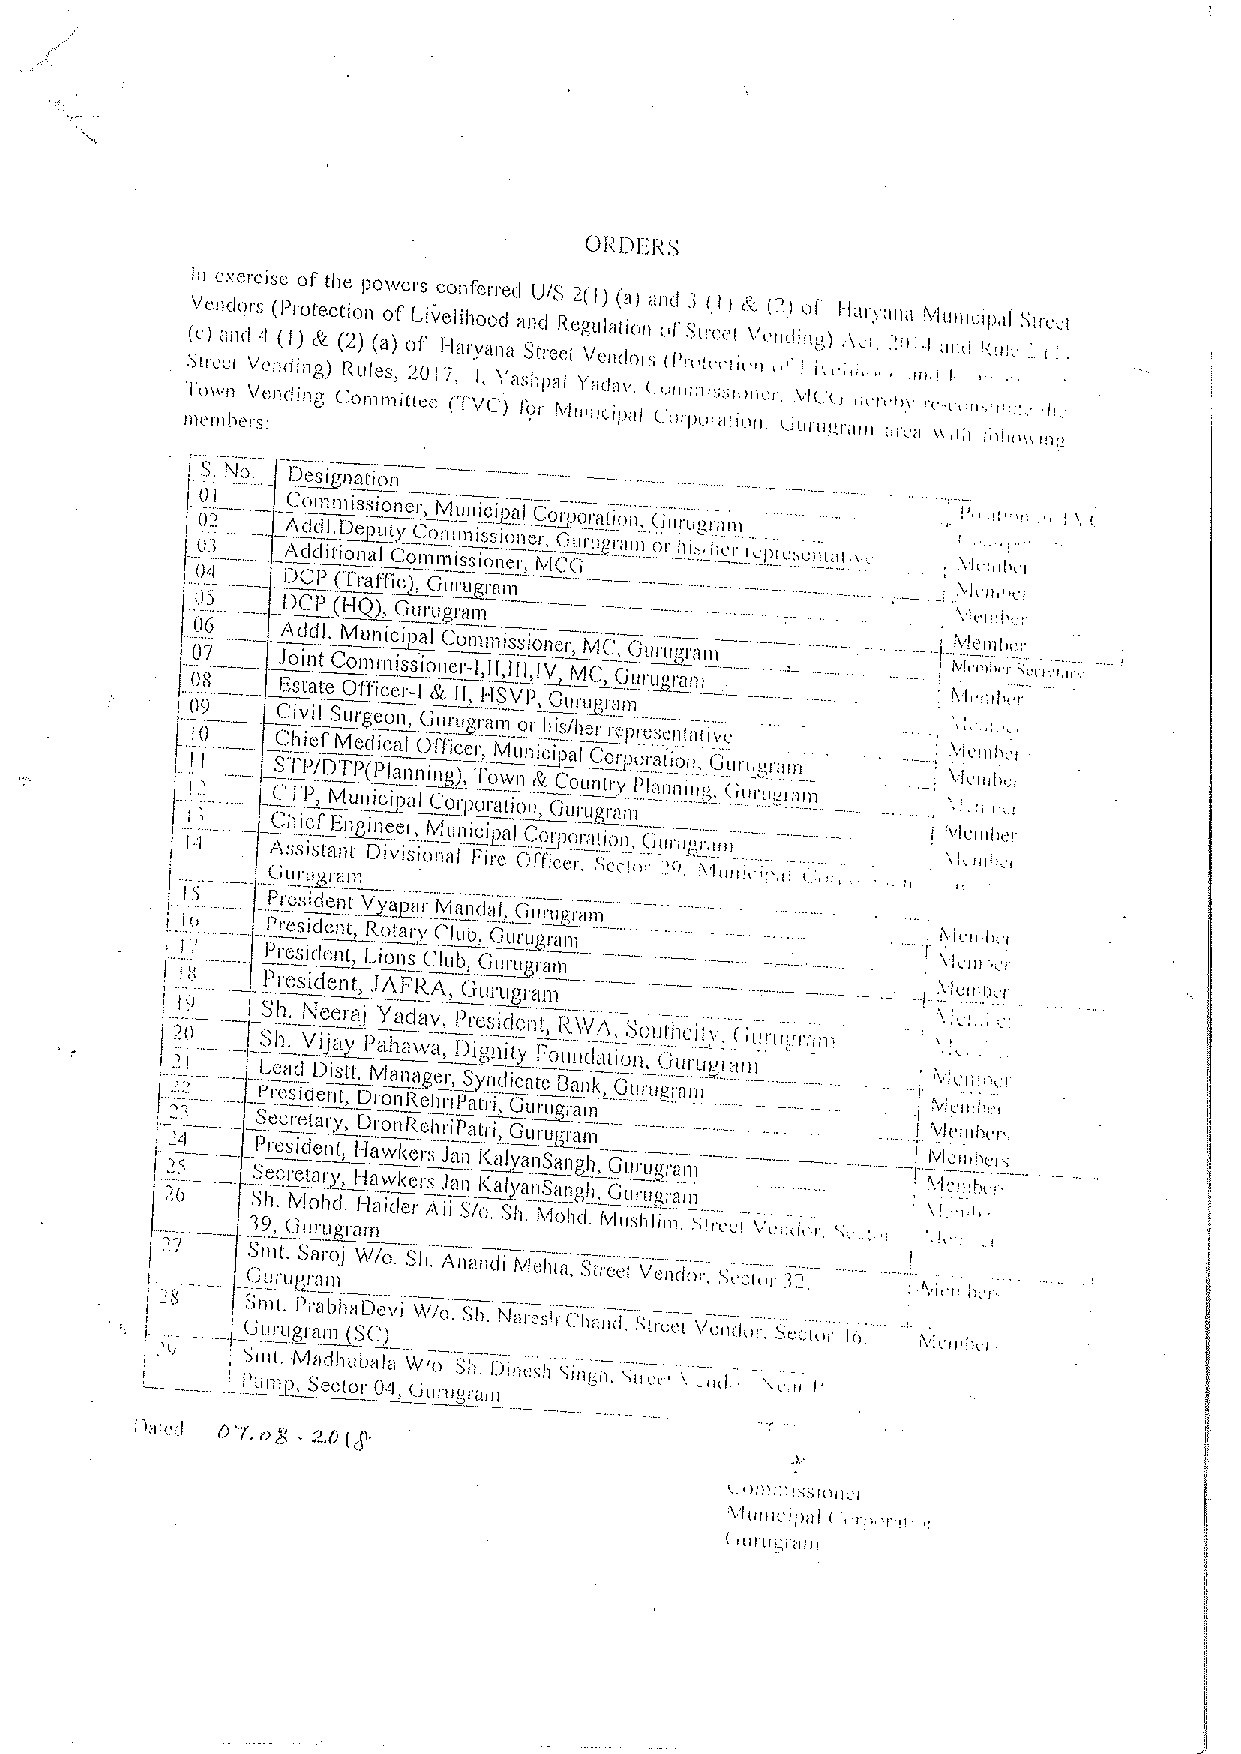
\includegraphics[width=5.1in]{Appendix6.pdf}
\end{figure}

%Appendix 5
\newpage
\section*{Appendix 5: List of TVC members as per TVC Meeting of August 2018}
\addcontentsline{toc}{section}{Appendix 5: List of TVC members as per TVC Meeting of August 2018}
\begin{figure}[h]
\centering
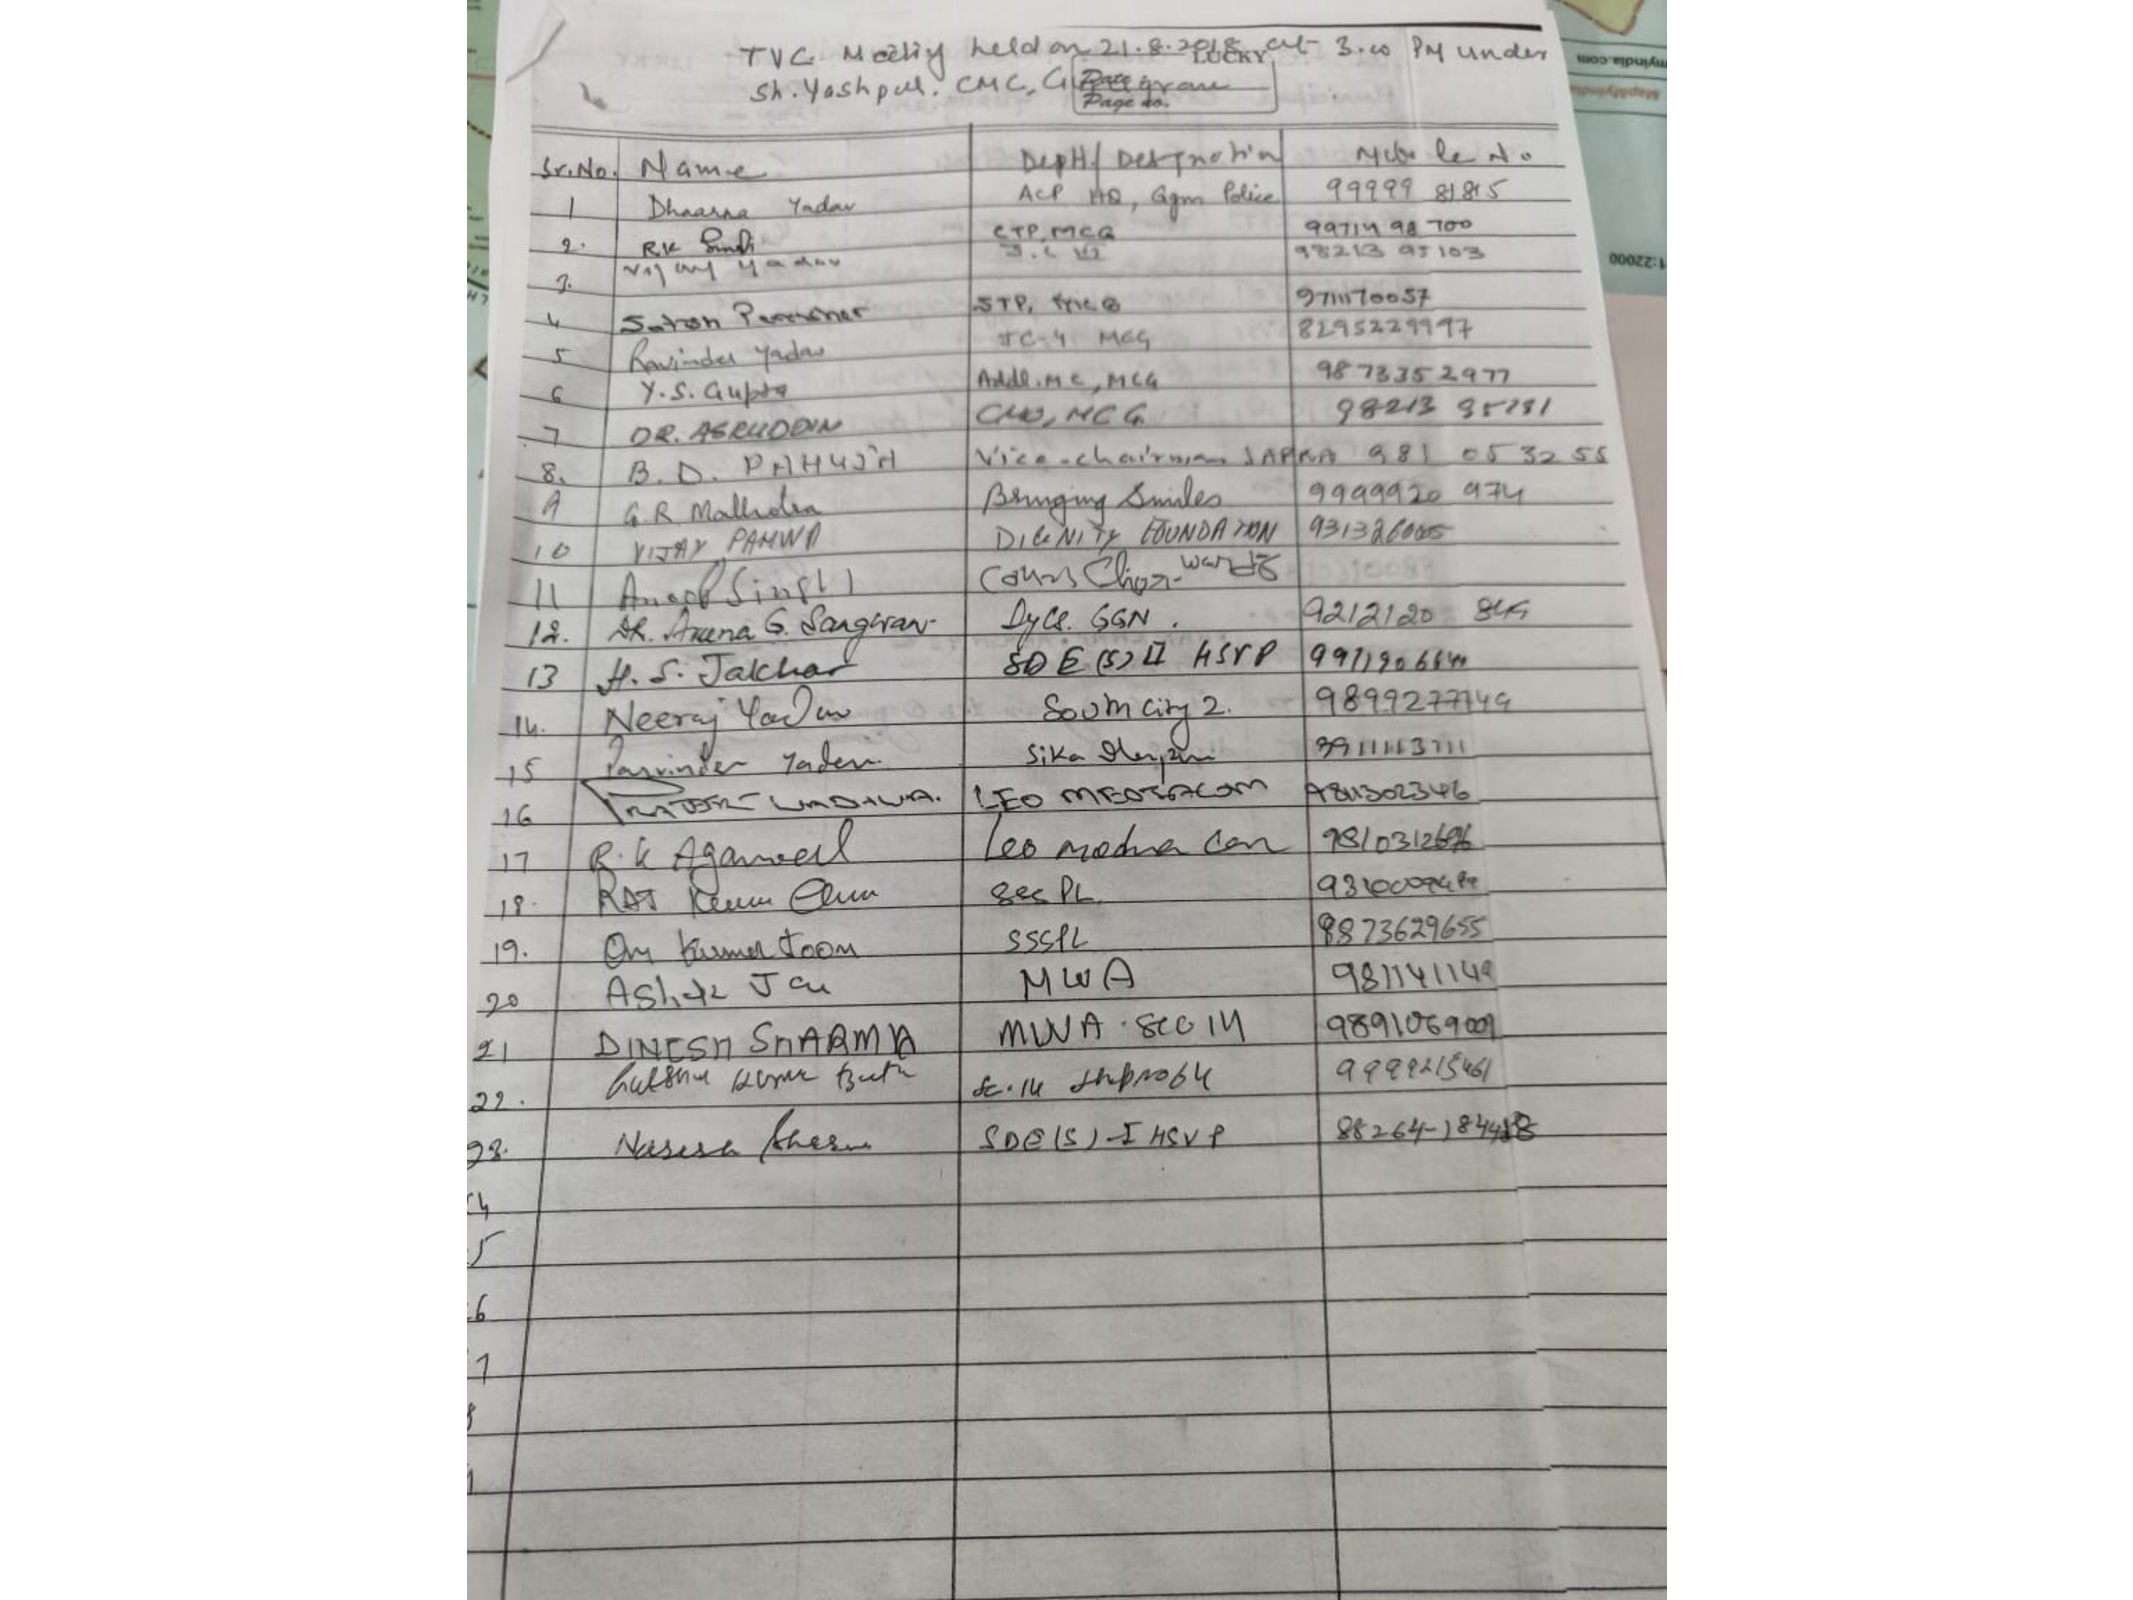
\includegraphics[width=7in]{ListofTVC.pdf}
\end{figure}

%Appendix 6
\newpage
\section*{Appendix 6: Receipt of Maintenance Fee Paid by \\Vendors}
\addcontentsline{toc}{section}{Appendix 6: Receipt of Maintenance Fee Paid by Vendors}
\begin{figure}[h]
\centering
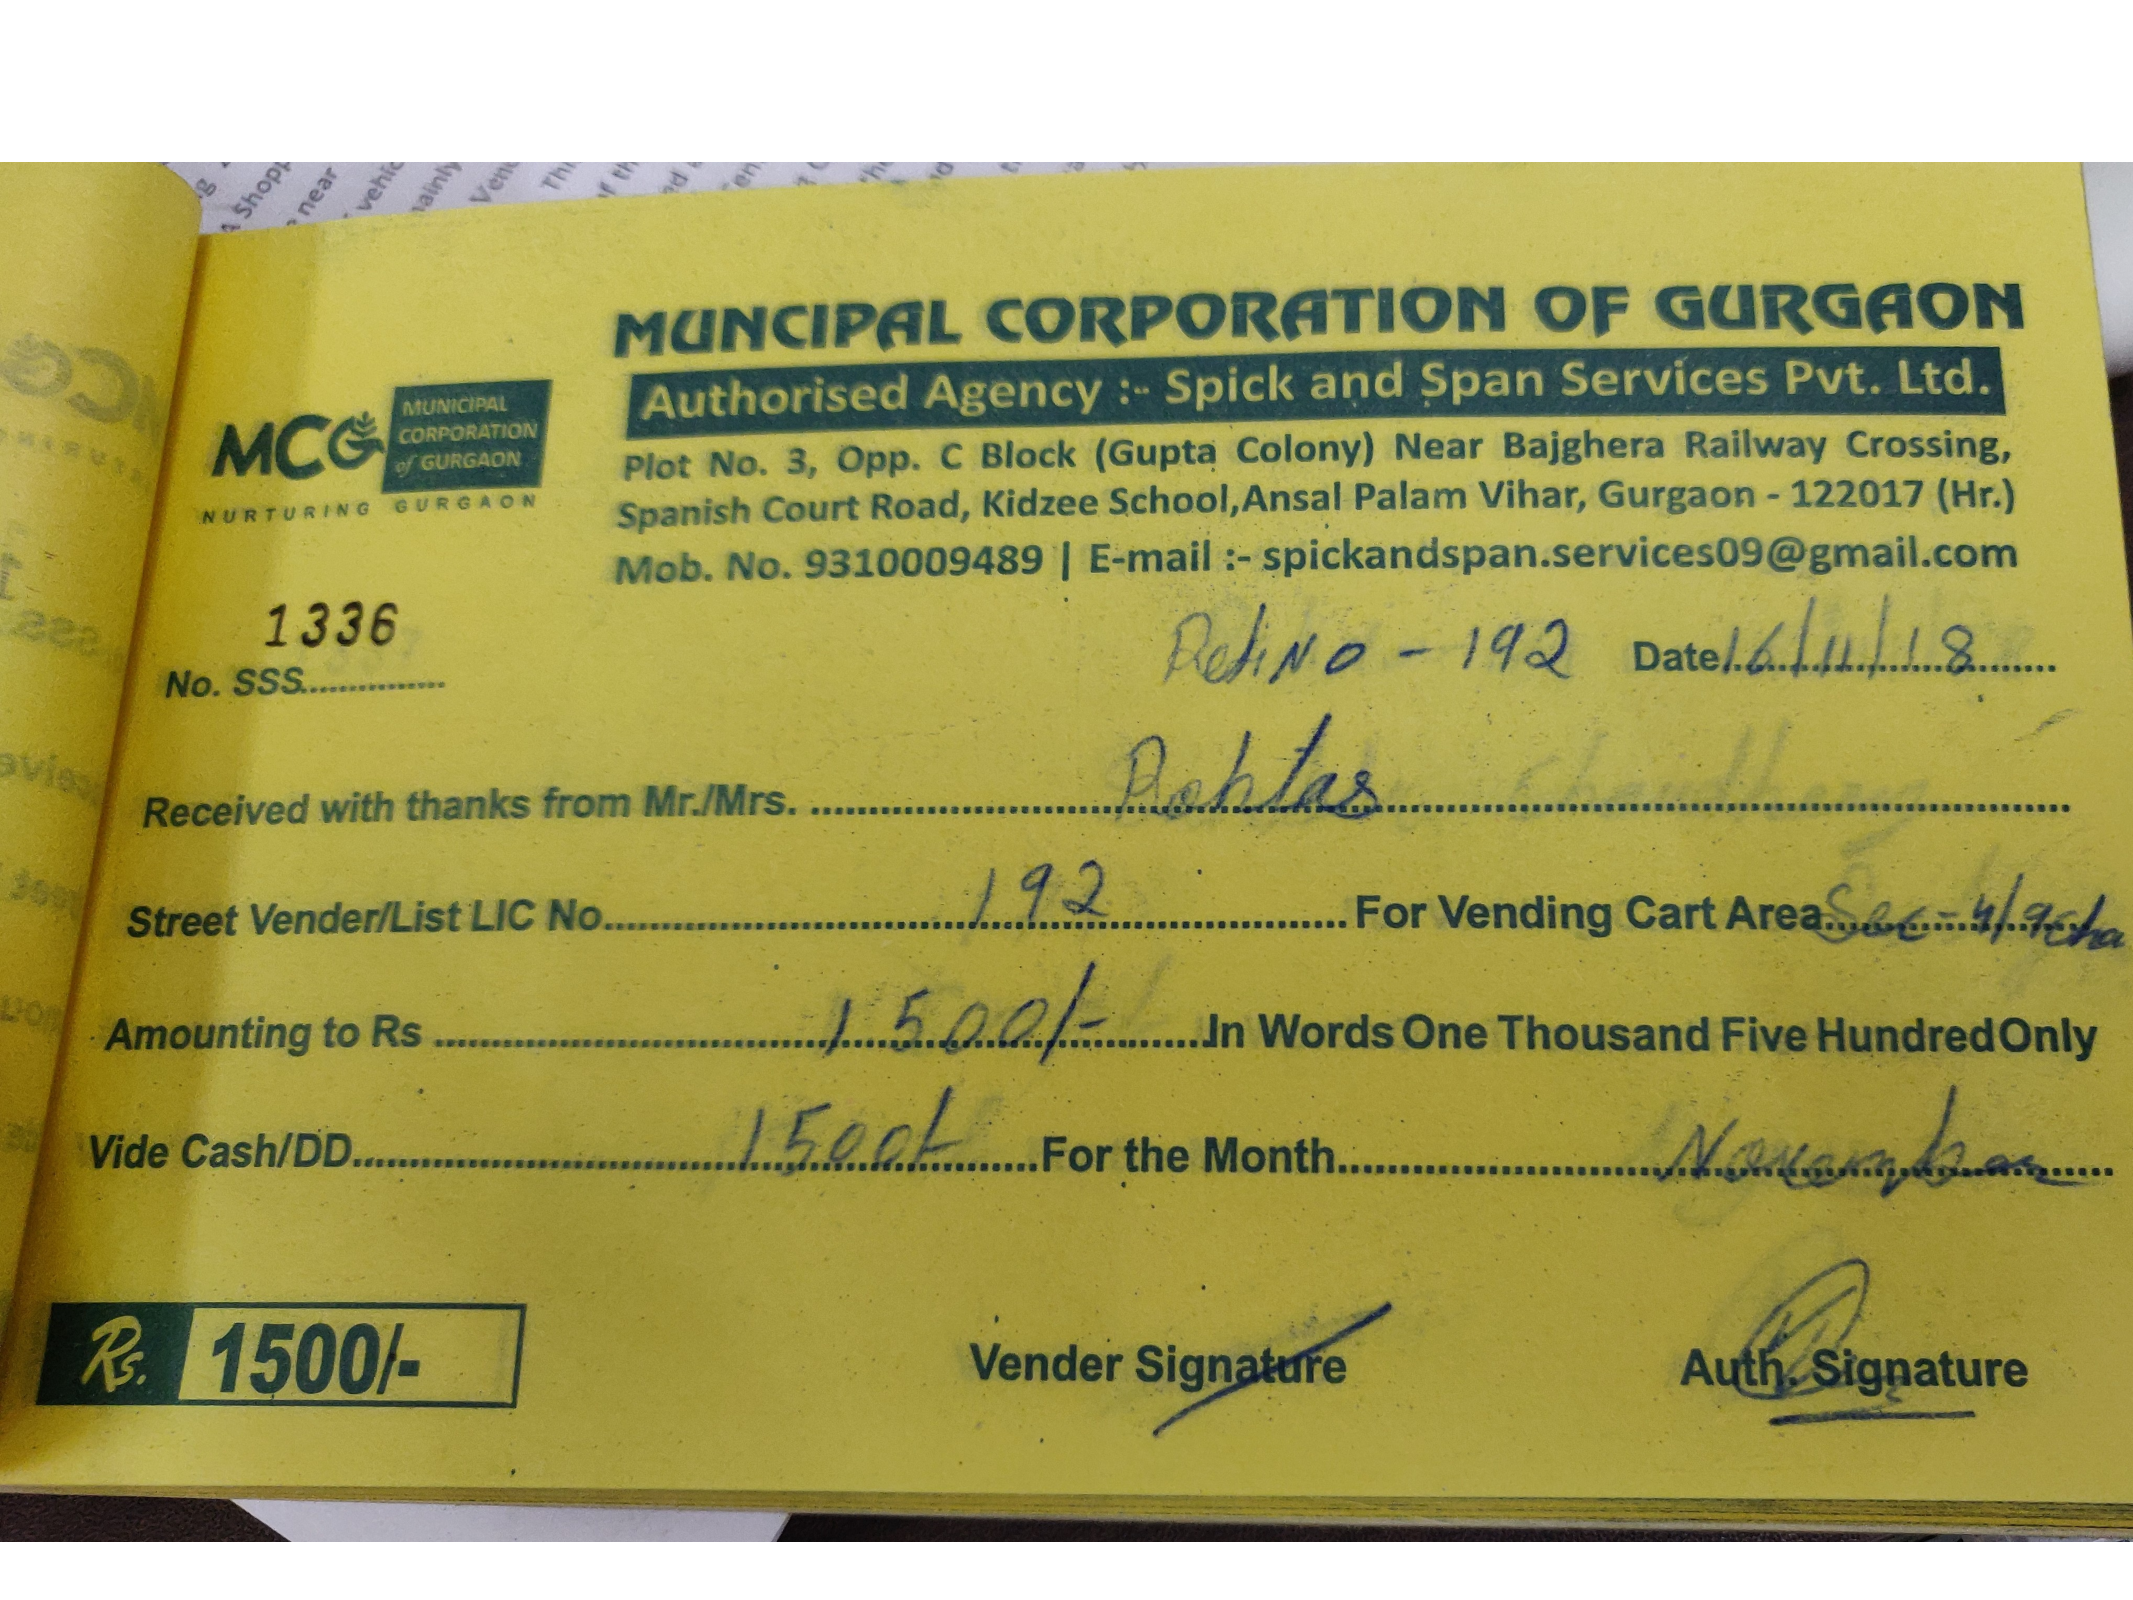
\includegraphics[width=6in]{Receipt1.pdf}
\end{figure}

%Appendix 7
\newpage
\section*{Appendix 7: Complaint Made By a Private Party to MCG against RWA}
\addcontentsline{toc}{section}{Appendix 7: Complaint Made By a Private Party to MCG against RWA}
\begin{figure}[h]
\centering

\includegraphics[height=5.5in]{Receipt2.pdf}
\end{figure}
%====================================================================
\end{document}
